\documentclass[a4paper,12pt]{article}
\usepackage[utf8]{inputenc}
\usepackage[T1]{fontenc}
\usepackage[french]{babel}
\usepackage{geometry}
\usepackage{lmodern}
\usepackage{hyperref}
\usepackage{titlesec}
\usepackage{tocloft}
\usepackage{xcolor}
\usepackage{graphicx}
\usepackage{float}



\geometry{margin=2.5cm}
\hypersetup{
    colorlinks=true,
    linkcolor=blue,
    urlcolor=blue,
    pdftitle={Rapport du projet PSID - LoveMyPet},
    pdfauthor={Imane Errahmani, Faiz Sadikou Adenle, Malek Messaoudi}
}

% Réduction légère des espaces verticaux dans la table des matières si besoin
\setlength{\cftbeforesecskip}{6pt}

\title{\textbf{Rapport du projet PSID }\\ \Large LoveMyPet}
\author{
    Imane Errahmani -- 43014746 \\
    Faiz Sadikou Adenle -- 42000139 \\
    Malek Messaoudi -- 42000319
}
\date{\today}

\begin{document}

\maketitle
\thispagestyle{empty}
\clearpage  % Sépare le titre et la table des matières

% Table des matières seule sur une page
\tableofcontents
\thispagestyle{empty}
\clearpage

% Contenu
\section {Présentation}

Ce rapport présente le projet \textbf{LoveMyPet}, réalisé dans le cadre du module PSID.

Ce document est une première version du rapport (v0.1) présentant le contexte, les membres de l’équipe, et une première synthèse des travaux réalisés.

\subsection {Problématique}

Chaque année, de nombreux animaux se retrouvent dans des refuges sans trouver de foyer. Malgré les efforts des associations, une part importante d’entre eux reste en attente d’adoption pendant des mois, ce qui entraîne des conséquences négatives pour leur bien-être. Cette problématique soulève une question essentielle : comment augmenter leurs chances d’être adoptés rapidement ?

Grâce aux données disponibles sur les profils des animaux (description, caractéristiques physiques, informations de santé, etc.), il devient possible d’analyser les éléments qui influencent le temps avant adoption. L’analyse de ces facteurs peut contribuer à mieux présenter les animaux et améliorer les stratégies de sensibilisation.

\subsection {Solution}

Pour répondre à cette problématique, nous avons développé le projet \textbf{LoveMyPet}, une étude basée sur l’analyse de données issues de la plateforme PetFinder. Le but est d’identifier les facteurs influençant la rapidité d’adoption des animaux en appliquant des techniques de data science et d’intelligence artificielle.

Notre solution se structure autour de plusieurs étapes clés :
\begin{itemize}
    \item Nettoyage et préparation des données (tabulaires, textuelles et visuelles).
    \item Visualisation exploratoire pour comprendre les tendances.
    \item Modélisation prédictive pour estimer la rapidité d’adoption.
    \item Interprétation et recommandations pour améliorer la présentation des profils.
\end{itemize}

Ce travail vise à outiller les refuges et associations d’adoption avec des indicateurs clairs et des leviers d’action pour favoriser des adoptions plus rapides et mieux ciblées.

\subsection{Public cible}

Le projet s’adresse principalement :
\begin{itemize}
    \item aux \textbf{associations de protection animale} qui cherchent à optimiser le placement des animaux de compagnie dans des foyers adaptés ;
    \item aux \textbf{refuges pour animaux}, qui doivent prendre des décisions rapides et informées pour augmenter les chances d’adoption ;
    \item aux \textbf{utilisateurs particuliers}, intéressés par l’adoption et désireux d’accéder à des recommandations personnalisées selon leurs préférences ou leur profil ;
    \item aux \textbf{organismes publics ou municipaux}, pour la gestion et l'amélioration des campagnes d'adoption sur leur territoire.
\end{itemize}

\subsection{Personas}

Pour mieux illustrer les besoins auxquels répond le projet, nous avons identifié deux personas types :

\vspace{1em}
\textbf{Persona 1 – Clara, bénévole dans un refuge}

\begin{itemize}
    \item \textbf{Âge} : 29 ans
    \item \textbf{Profession} : étudiante vétérinaire et bénévole
    \item \textbf{Besoins} : mieux comprendre pourquoi certains animaux mettent du temps à être adoptés ; savoir comment mettre en avant les bons critères dans les fiches descriptives.
    \item \textbf{Objectif} : améliorer les chances d’adoption des animaux les plus vulnérables.
\end{itemize}

\vspace{1em}
\textbf{Persona 2 – Marc, adoptant potentiel}

\begin{itemize}
    \item \textbf{Âge} : 45 ans
    \item \textbf{Profession} : enseignant
    \item \textbf{Besoins} : adopter un animal compatible avec son mode de vie et ses contraintes familiales.
    \item \textbf{Objectif} : accéder à des recommandations d’animaux faciles à adopter et correspondant à son environnement.
\end{itemize}

\section {Architecture métier}

\subsection {Frontend}

Le frontend du projet LoveMyPet a été développé en utilisant le framework \textbf{React} avec l’outil de bundling \textbf{Vite}, qui offre une configuration légère et un temps de compilation rapide. Pour le design et le style de l’interface, nous avons adopté \textbf{TailwindCSS}, un framework CSS utilitaire moderne, qui permet une personnalisation rapide et cohérente des composants graphiques.

L’interface utilisateur est conçue pour être simple, interactive et informative. Elle présente les graphiques de visualisation générés à partir des données analysées, notamment des diagrammes interactifs produits avec \textbf{Plotly.js}, qui permettent une navigation fluide et dynamique entre différentes catégories d’animaux, races, ou facteurs d’adoption. Des composants personnalisés comme les boutons de filtre ou les titres numérotés ont été développés pour guider la lecture et l’exploration des résultats.

\subsection {Backend}

Le backend est construit avec \textbf{FastAPI}, un framework Python moderne et performant, parfaitement adapté pour construire des API REST. Ce choix permet une communication fluide entre l’interface utilisateur et les données analysées en backend, tout en assurant un temps de réponse rapide.

Les données sont traitées avec \textbf{pandas}, une bibliothèque de référence pour la manipulation de données tabulaires en Python. Plusieurs endpoints ont été définis pour servir les résultats des analyses : répartition des types d’animaux, distribution des âges, top races stérilisées, impact de la stérilisation sur l’adoption rapide, etc.

Le backend se charge également du chargement et du nettoyage des jeux de données à partir de fichiers CSV, ainsi que de leur enrichissement par jointures avec des fichiers de correspondance (races, couleurs, états géographiques). Les analyses sont structurées pour fournir des réponses directement exploitables par les composants de visualisation du frontend.

\section {Pratiques de Collaboration et de DevOps Project}

\subsection {Management}

La gestion de projet s’est appuyée sur une méthodologie \textbf{Scrum}, adaptée aux projets étudiants et favorisant un développement itératif et collaboratif. Pour organiser les tâches, nous avons utilisé un tableau \textbf{Kanban} sur GitHub, permettant une répartition claire des responsabilités et une visualisation en temps réel de l’avancement du projet.

Nous avons également mis en place des réunions d’équipe hebdomadaires. Ces sessions régulières, similaires aux "stand-ups" Scrum, ont servi à faire le point sur les tâches réalisées, discuter des obstacles rencontrés et ajuster les priorités collectives. Cette dynamique a renforcé la cohésion de l’équipe et favorisé une communication continue.

\subsection {Versionnement}

Le versionnement du code a été centralisé via la plateforme \textbf{GitHub}, qui a permis un suivi rigoureux de l’évolution du projet. Grâce à l’utilisation des branches, commits et pull requests, chaque membre a pu travailler de manière autonome tout en maintenant l'intégrité du code commun. Les revues de code ont contribué à la détection précoce des erreurs et à la diffusion des bonnes pratiques au sein de l’équipe.

\subsection{Intégration Continue et Déploiement Continu}

Nous avons mis en place un pipeline d’intégration et de déploiement continu (\textbf{CI/CD}) en utilisant \textbf{GitHub Actions}. Chaque push sur la branche principale déclenche automatiquement un processus de build et de déploiement. Ce mécanisme garantit que les nouvelles fonctionnalités et corrections sont rapidement intégrées et accessibles.

Ce système permet de livrer plus fréquemment et avec davantage de fiabilité, tout en réduisant les risques d’erreur humaine. Le pipeline inclut des étapes de vérification de la qualité du code, ce qui renforce la stabilité de l’application avant chaque mise en production.

\subsection {Qualité du code}

Le contrôle qualité du code est assuré par l’outil d’analyse statique \textbf{Codacy}, intégré dans notre workflow GitHub. Codacy permet de détecter automatiquement les mauvaises pratiques de développement, les complexités inutiles ou les répétitions de code.

Nous avons personnalisé les règles d’analyse afin de coller aux standards définis par l’équipe, garantissant ainsi une uniformité dans le style de développement. Les rapports générés permettent de suivre en continu l’état du code et d’intervenir de manière proactive pour améliorer la robustesse du projet.

\section{Partie Data Analytique}

\subsection {Source de données}

Les données utilisées pour ce projet proviennent de la compétition Kaggle intitulée \textit{PetFinder.my Adoption Prediction}, accessible à l'adresse suivante :\\[0.5em]
\url{https://www.kaggle.com/competitions/petfinder-adoption-prediction}

\bigskip

\textbf{Nom du dataset} : PetFinder.my Adoption Prediction \\
\textbf{Source} : PetFinder.my, en partenariat avec Kaggle \\
\textbf{Pays d’origine des données} : Malaisie \\
\textbf{Date de mise à disposition} : 2019

\medskip

\noindent
\textbf{Contexte :} \\
Chaque jour, des millions d’animaux errants sont abandonnés ou euthanasiés par manque de foyers adoptants. PetFinder.my est la principale plateforme malaisienne de protection animale depuis 2008, avec une base de plus de 150 000 animaux enregistrés.

Cette plateforme collabore avec des ONG, des entreprises, des médias et des organisations internationales pour améliorer le bien-être animal. Dans ce contexte, les profils en ligne des animaux (textes descriptifs, caractéristiques des photos, etc.) ont un rôle majeur dans la rapidité d’adoption.

\medskip

\noindent
\textbf{Objectif de la compétition :} \\
L’objectif est de prédire la rapidité avec laquelle un animal est adopté, en fonction des métadonnées présentes dans son profil. Ces prédictions pourraient être intégrées dans des outils d’intelligence artificielle (IA), comme le \textit{Cuteness Meter}, pour conseiller les refuges sur l’optimisation des profils d’animaux. Cela permettrait d’accélérer les adoptions, d’éviter l’euthanasie, et d’améliorer significativement le bien-être animal à l’échelle mondiale.

\medskip

\noindent
\textbf{Intérêt pour le projet :} \\
Ce dataset constitue une base riche pour une analyse complète des facteurs d’adoption : il comprend des données tabulaires, textuelles et visuelles, et permet de tester des approches analytiques et prédictives variées.

\subsection {Présentation du dataset}


\paragraph{Structure du dataset :}
\begin{itemize}
    \item \texttt{train.csv} : Données d'entraînement (variables tabulaires et textuelles)
    \item \texttt{test.csv} : Données de test à prédire
    \item \texttt{sample\_submission.csv} : Exemple de fichier de soumission
    \item \texttt{breed\_labels.csv} : Identifiants et noms de races, ainsi que leur type (chien ou chat)
    \item \texttt{color\_labels.csv} : Noms associés à chaque code couleur
    \item \texttt{state\_labels.csv} : Noms associés à chaque code de région (Malaisie)
\end{itemize}

\paragraph{Détail des variables :}

Le fichier \texttt{train.csv} contient les variables suivantes, décrivant les caractéristiques des animaux disponibles à l’adoption sur la plateforme PetFinder.my :

\begin{itemize}
    \item \textbf{PetID} : Identifiant unique de chaque profil d’animal.
    \item \textbf{AdoptionSpeed} : Cible à prédire. Elle indique en combien de temps l’animal a été adopté.
          \begin{itemize}
              \item 0 : le jour même
              \item 1 : entre 1 et 7 jours
              \item 2 : entre 8 et 30 jours
              \item 3 : entre 31 et 90 jours
              \item 4 : non adopté après 100 jours
          \end{itemize}

    \item \textbf{Type} : Type d’animal (1 = chien, 2 = chat)
    \item \textbf{Name} : Nom de l’animal (vide si non renseigné)
    \item \textbf{Age} : Âge de l’animal (en mois)

    \item \textbf{Breed1} : Race principale de l’animal (identifiant numérique)
    \item \textbf{Breed2} : Race secondaire (si l’animal est croisé). Peut être 0.

    \item \textbf{Gender} : Sexe de l’animal
          \begin{itemize}
              \item 1 : Mâle
              \item 2 : Femelle
              \item 3 : Mixte (groupe d’animaux)
          \end{itemize}

    \item \textbf{Color1, Color2, Color3} : Couleurs dominantes (jusqu’à 3 couleurs)

    \item \textbf{MaturitySize} : Taille de l’animal à l’âge adulte
          \begin{itemize}
              \item 1 : Petite
              \item 2 : Moyenne
              \item 3 : Grande
              \item 4 : Très grande
              \item 0 : Non spécifié
          \end{itemize}

    \item \textbf{FurLength} : Longueur du pelage
          \begin{itemize}
              \item 1 : Court
              \item 2 : Moyenmercredi
              \item 3 : Long
              \item 0 : Non spécifié
          \end{itemize}

    \item \textbf{Vaccinated} : Statut de vaccination
          \begin{itemize}
              \item 1 : Oui
              \item 2 : Non
              \item 3 : Inconnu
          \end{itemize}

    \item \textbf{Dewormed} : Vermifugation effectuée ou non (1 = oui, 2 = non, 3 = inconnu)

    \item \textbf{Sterilized} : Animal stérilisé ou non (1 = oui, 2 = non, 3 = inconnu)

    \item \textbf{Health} : État de santé de l’animal
          \begin{itemize}
              \item 1 : En bonne santé
              \item 2 : Légèrement blessé
              \item 3 : Gravement blessé
              \item 0 : Non spécifié
          \end{itemize}

    \item \textbf{Quantity} : Nombre d’animaux représentés par le profil (souvent 1)

    \item \textbf{Fee} : Frais d’adoption demandés (0 = gratuit)

    \item \textbf{State} : État géographique de l’animal (en Malaisie)

    \item \textbf{RescuerID} : Identifiant du sauveteur ou refuge ayant publié l’annonce

    \item \textbf{VideoAmt} : Nombre de vidéos associées à l’animal

    \item \textbf{PhotoAmt} : Nombre de photos disponibles

    \item \textbf{Description} : Texte libre décrivant l’animal. Langues utilisées : anglais, malais, ou chinois.
\end{itemize}

\paragraph{Définition de la variable cible : \texttt{AdoptionSpeed}}
\begin{itemize}
    \item \textbf{0} : adopté le jour même
    \item \textbf{1} : adopté entre 1 et 7 jours
    \item \textbf{2} : adopté entre 8 et 30 jours
    \item \textbf{3} : adopté entre 31 et 90 jours
    \item \textbf{4} : non adopté après 100 jours
\end{itemize}

\paragraph{Données complémentaires :}
\begin{itemize}
    \item \textbf{Images} : Chaque animal possède une ou plusieurs photos, analysées via l'API Google Vision (annotation faciale, étiquettes, propriétés visuelles, textes).
    \item \textbf{Sentiment Analysis} : Les descriptions textuelles ont été soumises à l’API Google Natural Language pour extraire la tonalité émotionnelle (positif, neutre, négatif).
\end{itemize}

\subsection{Nettoyage et manipulation des Données}

\paragraph{Prétraitement des données}

La phase de prétraitement a été essentielle pour garantir la qualité et la fiabilité des analyses ultérieures. Elle s’est déroulée selon les étapes suivantes :

\subparagraph{Contrôle de qualité}
\begin{itemize}
    \item \textbf{Détection des doublons} : Aucune duplication n’a été identifiée dans le jeu de données, ce qui écarte les biais potentiels liés à la redondance des profils.
    \item \textbf{Gestion des valeurs manquantes} : Une vérification systématique a révélé l'absence de valeurs nulles. Il n’a donc pas été nécessaire de procéder à une imputation ou à l’exclusion d’observations.
\end{itemize}

\subparagraph{Suppression des variables non pertinentes}
Certaines variables ont été supprimées, car jugées non informatives ou peu pertinentes pour l’objectif de prédiction de la rapidité d’adoption :
\begin{itemize}
    \item \textbf{VideoAmt} : Le nombre de vidéos associées aux animaux était quasi constant, et donc non discriminant.
    \item \textbf{State} : La localisation (État en Malaisie) ne présentait pas de corrélation significative avec la variable cible \textit{AdoptionSpeed}.
    \item \textbf{Name} : Souvent absente ou trop spécifique, cette variable n'apportait pas de valeur prédictive généralisable.
    \item \textbf{Description} : Bien que potentiellement riche en information, ce champ non structuré n’a pas été exploité dans cette première version, faute de traitement NLP prévu.
    \item \textbf{RescuerID} : Identifiant du sauveteur, non pertinent pour l’analyse, car non directement lié aux caractéristiques des animaux.
\end{itemize}

\subparagraph{Format des données}

Le jeu de données était déjà majoritairement numérique. Les variables catégorielles comme \textit{Breed} ou \textit{Color} sont fournies sous forme d’identifiants entiers, avec les correspondances disponibles dans des fichiers annexes fournis par Kaggle (\texttt{breed\_labels.csv}, \texttt{color\_labels.csv}, etc.).

\subparagraph{Encodage et transformations}

Aucune transformation supplémentaire (encodage one-hot, normalisation, standardisation) n’a été nécessaire à ce stade. Le format initial des données était directement exploitable pour les modèles de machine learning tabulaire.

\subparagraph{Résultat}

À l’issue de cette phase, un jeu de données nettoyé et allégé a été obtenu, contenant uniquement les variables jugées pertinentes. Ce jeu est enregistré dans le fichier \texttt{data\_clean.csv} et constitue la base des analyses exploratoires et des modèles prédictifs développés par la suite.

\subsection{Les graphiques présentés}

Nous avons intégré plusieurs visualisations interactives dans notre tableau de bord afin d’analyser les facteurs influençant l’adoption rapide des animaux. Ces graphiques sont construits dynamiquement en React à l’aide de la bibliothèque Plotly.js, et les données sont récupérées depuis notre API backend.


\paragraph{Adoption Animale : Les Clés pour une Adoption Rapide des Chiens et Chats}

Ce graphique en barres empilées présente la répartition des adoptions selon le délai (le jour même, entre 1 et 7 jours, entre 8 et 30 jours), en fonction de plusieurs caractéristiques : taille à maturité, état de santé, vaccination, vermifugation et stérilisation. L'analyse est segmentée par type d’animal (chiens ou chats).

\begin{itemize}
    \item Chez les chiens, les individus en bonne santé, vermifugés et de taille moyenne sont les plus rapidement adoptés.
    \item Les chiens non stérilisés sont adoptés plus rapidement que ceux qui le sont, ce qui peut refléter certaines préférences culturelles ou un manque d'information sur les bénéfices de la stérilisation.
    \item La vaccination n’a pas un impact majeur sur la rapidité d’adoption chez les chiens.
    \item Chez les chats, les mêmes tendances s’observent : la santé générale et la vermifugation influencent positivement l’adoption rapide.
    \item Cependant, un paradoxe apparaît : les chats non vaccinés sont adoptés plus vite que les vaccinés. Cela pourrait être lié à l'âge (les plus jeunes n’étant pas encore vaccinés) ou à des perceptions erronées.
    \item La stérilisation a également un effet inverse aux attentes : les chats non stérilisés sont adoptés plus rapidement.
\end{itemize}

En résumé, les facteurs liés à la santé visible jouent un rôle crucial dans l’adoption rapide. Toutefois, certaines perceptions des adoptants – notamment sur la stérilisation et la vaccination – semblent aller à l’encontre des recommandations vétérinaires, d’où l’intérêt de renforcer la sensibilisation.


\paragraph{Analyse du lien entre l’âge et la non-vaccination}

Ce graphique en barres illustre le nombre d’animaux non vaccinés selon leur tranche d’âge. Il fait suite à l'observation précédente d'un nombre élevé d’animaux proposés à l’adoption sans vaccination, et vise à mieux comprendre cette situation en l’associant à l’âge des animaux.

\begin{itemize}
    \item Une large majorité des animaux non vaccinés ont moins de 10 mois, avec un total de \textbf{6580 cas}, soit une concentration très marquée dans cette première tranche.
    \item Les chiffres chutent rapidement dans les groupes suivants : \textbf{383 individus} entre 11 et 20 mois, puis \textbf{134} entre 21 et 30 mois, et seulement quelques dizaines au-delà.
    \item Cela s’explique par le fait que de nombreux animaux sont proposés à l’adoption très jeunes, souvent avant l’âge recommandé pour administrer les premiers vaccins.
    \item Ce phénomène reflète aussi une préférence des adoptants pour les chiots ou chatons, qui n’ont pas encore suivi de protocole vaccinal complet.
    \item Il est également possible que certains refuges laissent volontairement cette responsabilité aux adoptants, dans le cadre d’accords personnalisés ou pour des raisons économiques.
\end{itemize}

En conclusion, la forte proportion d’animaux non vaccinés s’explique avant tout par leur jeune âge au moment de la mise à l’adoption, et ne constitue pas nécessairement un indicateur de négligence ou de mauvaise prise en charge.

\paragraph{Est-ce que le nombre de photos postées augmente la vitesse d’adoption ?}

Ce graphique combine deux analyses complémentaires : la première présente la vitesse d’adoption par groupe de photos, la seconde met en lumière le nombre total d’animaux adoptés et non adoptés selon le nombre de photos disponibles.

\begin{itemize}
    \item Les animaux avec 0 à 5 photos sont ceux qui sont adoptés le plus rapidement, notamment le jour même ou dans la première semaine.
    \item Lorsque le nombre de photos augmente (au-delà de 10), la rapidité d’adoption diminue fortement. Les adoptions immédiates deviennent rares, voire inexistantes pour les groupes avec plus de 20 photos.
    \item Ce phénomène suggère un possible effet de saturation ou de surcharge cognitive : trop d’images rendraient la décision plus difficile à prendre.
    \item Malgré leur forte visibilité, les animaux du groupe “0-5 photos” représentent aussi le plus grand nombre de non-adoptés après 100 jours, ce qui indique qu’un faible nombre de photos n’est pas un gage de succès à long terme.
    \item Les groupes intermédiaires (6-10 photos) semblent offrir un meilleur équilibre entre visibilité et efficacité d’adoption.
\end{itemize}

Ainsi, un nombre modéré de photos (entre 5 et 10) apparaît comme le plus efficace pour favoriser l’adoption rapide. Au-delà, il devient essentiel de miser sur la qualité et la pertinence des images, ainsi que sur un renouvellement régulier des visuels.

\paragraph{Analyse de la vitesse d’adoption par genre et par taille}

Ce graphique en radar explore l’influence du genre (mâle ou femelle) sur la vitesse d’adoption des animaux, tout en intégrant un filtre par taille (petit, moyen, grand, très grand). Il permet de comparer visuellement les comportements d’adoption selon ces deux caractéristiques.

\begin{itemize}
    \item Les femelles sont généralement adoptées plus rapidement que les mâles, surtout pour les petites et moyennes tailles.
    \item Pour les grandes tailles, les mâles deviennent plus nombreux à être adoptés, notamment après les premiers jours, et ils dominent aussi parmi les animaux non adoptés.
    \item En ce qui concerne les très grandes tailles, les adoptions sont initialement équilibrées entre les sexes, mais les mâles finissent par être plus représentés.
    \item La taille de l’animal semble jouer un rôle dans les préférences d’adoption, probablement lié à l’image projetée (compagnon affectueux pour les petits animaux, protecteur ou utilitaire pour les grands).
    \item Ces différences pourraient refléter des stéréotypes ou attentes comportementales selon le genre et la taille.
\end{itemize}

Ce graphique suggère que des stratégies différenciées selon le sexe et la taille des animaux pourraient améliorer les chances d’adoption, en jouant sur les perceptions et les attentes des futurs adoptants.

\paragraph{ Plus c’est court, plus c’est adopté ? Étude sur la rapidité d’adoption selon la fourrure}

Ce graphique en camembert met en évidence la répartition des adoptions rapides (dans les 7 premiers jours) selon la longueur de la fourrure des animaux : courte, moyenne ou longue. Il permet d’observer l’impact d’un critère physique souvent négligé mais potentiellement déterminant dans le processus d’adoption.

\begin{itemize}
    \item Les animaux à poil court sont adoptés le plus rapidement, représentant 52{,}7\% des adoptions rapides. Ils bénéficient d’une image de facilité d’entretien (moins de toilettage, moins de poils), ce qui séduit les adoptants.
    \item Les animaux à poil mi-long arrivent ensuite avec 38{,}5\% des adoptions rapides. Bien qu’ils soient un peu moins prisés que les poils courts, ils restent dans une proportion significative.
    \item Les animaux à poil long ne représentent que 8{,}9\% des adoptions rapides. Leur entretien plus contraignant (brossage, risque de nœuds) pourrait expliquer cette faible attractivité.
    \item La fourrure est donc un facteur non négligeable dans la prise de décision : elle renvoie à des représentations pratiques (entretien, propreté) et parfois esthétiques.
    \item Cette analyse peut aider les refuges à adapter leur communication, en valorisant les aspects positifs des animaux à fourrure longue, souvent moins rapidement adoptés.
\end{itemize}

Ce critère simple mais visuellement marquant joue donc un rôle dans la perception initiale des adoptants, influençant directement la vitesse d’adoption.

\paragraph{Comprendre la stérilisation animale : une question d’âge et de genre}

Cette double visualisation propose une lecture croisée des comportements de stérilisation chez les chiens et les chats, en distinguant les sexes et les tranches d’âge. L’objectif est de comprendre si certaines populations animales sont plus souvent stérilisées que d’autres, et à quel moment cela intervient dans leur vie.

\begin{itemize}
    \item Le premier graphique présente le nombre d’animaux stérilisés et non stérilisés selon leur sexe. On observe une nette prédominance des animaux non stérilisés, en particulier chez les mâles.
    \item Les femelles, quant à elles, sont davantage ciblées par les campagnes de stérilisation, probablement pour des raisons liées à la reproduction et à la gestion des portées.
    \item Le second graphique, en ligne, illustre l’évolution du pourcentage de stérilisation en fonction de l’âge. Les taux augmentent avec le temps, confirmant que les animaux sont rarement stérilisés très jeunes.
    \item Chez les chiens, la stérilisation progresse de manière plus linéaire, tandis que chez les chats, la courbe est plus abrupte, suggérant une intervention plus précoce.
    \item L'écart entre mâles et femelles est aussi plus marqué chez les chiens, là où chez les chats, les différences de genre sont moins prononcées.
\end{itemize}

Ces résultats révèlent l’existence de pratiques différenciées selon les espèces, les sexes et les âges. Ils peuvent servir de base pour ajuster les stratégies de sensibilisation et les politiques vétérinaires, en favorisant une stérilisation plus équitable et ciblée.

\paragraph{Impact de la stérilisation sur l’adoption rapide selon la race}

Ce graphique à barres groupées compare le taux d’adoption rapide des animaux stérilisés et non stérilisés pour les 10 races les plus fréquentes, avec un filtre par type d’animal (chien ou chat) et par pureté de race.

\begin{itemize}
    \item Les animaux stérilisés ont généralement un meilleur taux d’adoption rapide. Cela est perçu comme un indicateur de soin et de responsabilité.
    \item Les races populaires (Labrador, Poodle, Shih Tzu) montrent un effet amplifié : la combinaison stérilisation + pureté de race améliore fortement les chances d’adoption.
    \item Pour les races controversées (Pit Bull, Bull Terrier), la stérilisation a un effet modéré, souvent éclipsé par les stéréotypes négatifs.
    \item Chez les races mixtes, la stérilisation est le principal levier d’amélioration, car la pureté de race n’est pas perçue comme un avantage.
\end{itemize}

L’analyse croisée des effets montre que la stérilisation et la race pure forment un binôme stratégique pour l’adoption rapide. Toutefois, une communication ciblée reste nécessaire pour certaines races stigmatisées.

\paragraph{Top 10 Races Pures et Mixtes les Plus Rapides à Être Adoptées}

Ce graphique à barres présente, pour chaque type d’animal (chiens ou chats), les 10 races pures (en vert) et 10 races mixtes (en rouge) adoptées le plus rapidement. L’indicateur utilisé est la vitesse moyenne d’adoption (0 = adopté le jour même, 4 = non adopté après 100 jours).

\begin{itemize}
    \item \textbf{Chez les chiens}, certaines races mixtes surpassent même les pures : le Maltais mixte (1,30) et le Cocker Spaniel mixte (1,50) sont plus rapidement adoptés que leurs homologues de race pure.
    \item Les races pures restent dominantes dans certains cas : Basset Hound (1,60), Border Collie (1,69) et Pug (1,71) témoignent d’un fort attrait.
    \item \textbf{Chez les chats}, les races mixtes sont clairement en tête : Ragdoll mixte (1,70) et Maine Coon mixte (1,75) sont les plus rapidement adoptées, surpassant les versions pures de ces races.
    \item Des races pures comme le Domestic Long Hair (1,70) et le Russian Blue (1,91) conservent néanmoins un bon taux d’adoption.
    \item \textbf{Comparaison chiens vs chats} : la pureté de race semble jouer un rôle plus fort chez les chiens que chez les chats, pour lesquels les races mixtes sont davantage valorisées.
\end{itemize}

Cette analyse montre que les préférences des adoptants varient selon l’espèce. Tandis que les races pures bénéficient d’un capital de confiance chez les chiens, les chats mixtes séduisent davantage, possiblement pour leur originalité perçue. Les refuges peuvent adapter leur communication selon ces tendances pour améliorer les chances d’adoption rapide.

\paragraph{Analyse interactive des facteurs de non-adoption}

Ce graphique radar met en évidence les caractéristiques typiques des animaux qui ne trouvent pas d’adoptants après plus de 100 jours. Il permet de visualiser les variables influençant négativement l’adoption : âge plus élevé, frais d’adoption élevés, nombre de photos réduit, pelage et taille standards.

\begin{itemize}
    \item Les animaux non adoptés ont en moyenne 13,7 mois, ce qui les rend moins attractifs que les jeunes chiots ou chatons.
    \item Un faible nombre de photos (en moyenne 3,32) réduit l’impact émotionnel des profils.
    \item Les frais d’adoption supérieurs à 21 MYR peuvent décourager les potentiels adoptants.
    \item La santé ne semble pas être un facteur majeur de rejet : la majorité sont en bonne santé.
\end{itemize}

L’interprétation globale suggère que l’amélioration de la présentation visuelle (photos, descriptions, vidéos) ainsi qu’une stratégie tarifaire adaptée pourraient significativement accroître les chances d’adoption.

\textcolor{red}{Tous les graphes sont disponibles sur notre site dans la vidéo de démonstration ainsi que sur GitHub. Vous trouverez les liens vers ces deux ressources dans le fichier \texttt{lien\_code\_source.txt}.}

\section{Analyse statistique}


\subsection{Résultats de Kaggle : une base de comparaison}

Bien que ce jeu de données ait déjà été exploité dans le cadre d’une compétition organisée sur \textit{Kaggle}, les résultats obtenus par les participants ont plafonné autour d'une précision de 45\%, malgré l’utilisation de modèles avancés et d’approches algorithmiques sophistiquées. Ce plafond de performance interroge : est-ce dû à la qualité des données, à des facteurs structurels ignorés, ou à des limites des modèles utilisés ?

Ce projet propose de prendre le problème à la racine : plutôt que de chercher uniquement à améliorer les scores, il s'agit de comprendre pourquoi ces performances stagnent, en explorant en profondeur les données, les variables et les relations cachées, ce que les modèles ont peut-être raté. L’objectif est double : mieux expliquer le phénomène d’adoption, et envisager des pistes concrètes pour faire mieux.

\subsection{Analyse des valeurs aberrantes (outliers)}

Les boxplots ont été utilisés pour analyser la distribution des variables du jeu de données. Pour la variable continue \textbf{Age}, des valeurs aberrantes dépassant 150 (jusqu'à 250) ont été détectées. Ces données aberrantes ont été supprimées afin d'améliorer la qualité des données et d'éviter un impact négatif sur le modèle.

Les autres variables, telles que \textbf{Gender}, \textbf{Color1}, \textbf{Color2}, \textbf{Color3}, \textbf{MaturitySize}, \textbf{FurLength}, \textbf{Vaccinated} et \textbf{Dewormed}, sont des variables catégoriques codées numériquement (par exemple, de 1 à 7 pour \texttt{Color1}). Les points isolés observés dans leurs boxplots correspondent à des catégories moins fréquentes, ce qui est attendu pour des variables catégoriques, et ne constitue donc pas des anomalies.

Cette analyse a permis de confirmer la cohérence globale des données après nettoyage.

\begin{figure}[H]
    \centering
    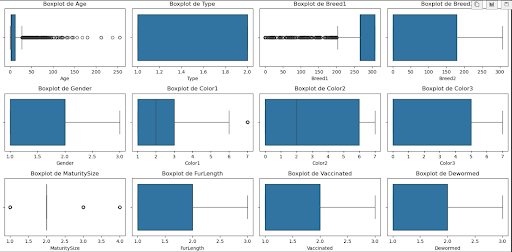
\includegraphics[width=0.65\textwidth]{boxplot_age_outliers.png}
    \caption{Boxplot illustrant les valeurs aberrantes}
    \label{fig:outliers_age}
\end{figure}

\subsection{Premier test : Régression logistique multiclasse}

Pour évaluer la cohérence de nos données et obtenir une première estimation des performances, nous avons entraîné un modèle de \textbf{régression logistique multiclasse}. Cette étape visait également à situer nos résultats par rapport au concours Kaggle, où une précision de \textbf{0{,}45} avait été atteinte.

L'entraînement a été réalisé en utilisant les variables suivantes comme descripteurs : \texttt{Type}, \texttt{Age}, \texttt{Breed1}, \texttt{Breed2}, \texttt{Gender}, \texttt{Color1}, \texttt{Color2}, \texttt{Color3}, \texttt{MaturitySize}, \texttt{FurLength}, \texttt{Vaccinated}, \texttt{Dewormed}, \texttt{Sterilized}, \texttt{Health}, \texttt{Fee}, \texttt{VideoAmt} et \texttt{PhotoAmt}. La variable cible à prédire est \texttt{AdoptionSpeed}, prenant des valeurs entières de 0 à 4.

\begin{table}[ht]

    \centering

    \begin{tabular}{|c|c|}

        \hline

        \textbf{Métrique}        & \textbf{Valeur}                   \\ \hline

        MSE (Mean Squared Error) & 2,2317                            \\ \hline

        Biais                    & 1,9788                            \\ \hline

        Variance                 & 0,2529                            \\ \hline

        Précision moyenne        & 0,2699                            \\ \hline

        Problème identifié       & Sous-apprentissage (Underfitting) \\ \hline
    \end{tabular}

    \caption{Résumé des performances du modèle de régression logistique}

\end{table}

Le modèle présente un \textbf{MSE de 2{,}2317}, un \textbf{biais élevé de 1{,}9788} et une \textbf{variance relativement faible de 0{,}2529}, indiquant un problème de \textbf{sous-apprentissage} (\textit{underfitting}). La précision moyenne s'élève à environ \textbf{26{,}99\%}, soulignant la difficulté du modèle à capturer les relations présentes dans les données.

\begin{figure}[H]

    \centering

    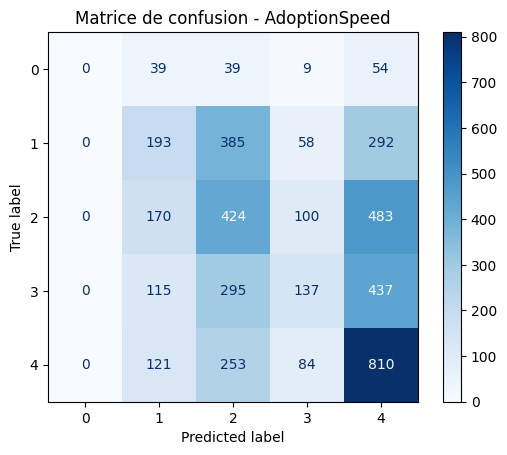
\includegraphics[width=0.75\textwidth]{matrice_confusion_logreg.png}

    \caption{Matrice de confusion obtenue avec la régression logistique}

    \label{fig:confusion_logreg}

\end{figure}

Le rapport de classification obtenu est présenté dans le tableau suivant :

\begin{table}[h]

    \centering

    \begin{tabular}{|c|c|c|c|c|}

        \hline

        \textbf{Classe} & \textbf{Précision}       & \textbf{Rappel} & \textbf{F1-score} & \textbf{Support} \\ \hline

        0               & 0,00                     & 0,00            & 0,00              & 141              \\ \hline

        1               & 0,30                     & 0,21            & 0,25              & 928              \\ \hline

        2               & 0,30                     & 0,36            & 0,33              & 1177             \\ \hline

        3               & 0,35                     & 0,14            & 0,20              & 984              \\ \hline

        4               & 0,39                     & 0,64            & 0,48              & 1268             \\ \hline

        \textbf{Total}  & \textbf{Accuracy = 0,35} &                 &                   & \textbf{4498}    \\ \hline
    \end{tabular}

    \caption{Rapport de classification après entraînement du modèle}

\end{table}

\vspace{0.5cm}

\noindent

Moyennes globales :

\begin{itemize}

    \item Macro moyenne : précision = 0,27 ; rappel = 0,27 ; F1-score = 0,25

    \item Moyenne pondérée : précision = 0,33 ; rappel = 0,35 ; F1-score = 0,32

\end{itemize}

L'analyse du rapport de classification et de la matrice de confusion confirme le faible pouvoir prédictif du modèle. La classe \textbf{0} n'est \textbf{jamais prédite}, avec une précision et un rappel nuls. Les autres classes présentent également des résultats faibles, comme l'illustrent des \textit{f1-scores} bas et déséquilibrés. L'exactitude globale du modèle est d’environ \textbf{35\%}, bien en deçà des attentes.

Par ailleurs, la distribution des classes montre un important déséquilibre :

\begin{figure}[H]

    \centering

    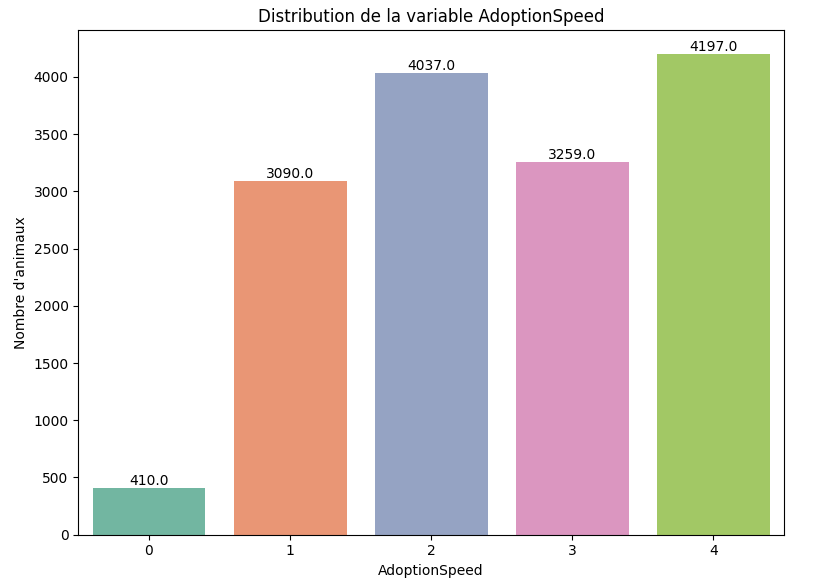
\includegraphics[width=0.7\textwidth]{adoption_speed_distribution.png}

    \caption{Répartition des animaux selon la vitesse d’adoption (AdoptionSpeed)}

    \label{fig:adoption_speed}

\end{figure}

On observe notamment que la classe \textbf{4} (animaux non adoptés après 100 jours) est majoritaire avec plus de 4 000 individus, alors que la classe \textbf{0} (adoption immédiate) compte  de 450 exemples. Ce déséquilibre important complique la tâche du modèle, en particulier pour la prédiction des classes minoritaires.



\subsection{Analyse après duplication de la classe 0}
 
Après avoir multiplié les occurrences de la classe 0 par 7 pour atteindre environ 3 090 exemples, nous avons réentraîné le modèle de régression logistique. Voici les résultats obtenus.
 
\begin{table}[h]

\centering

\begin{tabular}{|c|c|}

\hline

\textbf{Métrique} & \textbf{Valeur} \\ \hline

MSE & 3,6941 \\ \hline

Biais & 3,3316 \\ \hline

Variance & 0,3626 \\ \hline

Précision moyenne (validation croisée) & 0,2945 \\ \hline

\end{tabular}

\caption{Résultats globaux du modèle après duplication de la classe 0}

\end{table}
 
La duplication de la classe 0 a permis une légère amélioration globale : la précision moyenne atteint 29,45\%, avec une erreur quadratique moyenne (MSE) de 3,6941. Le biais reste élevé (3,3316), traduisant toujours un problème de sous-apprentissage. La variance demeure faible (0,3626), indiquant un modèle stable sans surapprentissage.
 
\bigskip
 
Le rapport de classification par classe montre une amélioration ciblée sur la classe 0 :
 
\begin{table}[h]

\centering

\begin{tabular}{|c|c|c|c|}

\hline

\textbf{Classe} & \textbf{Précision} & \textbf{Rappel} & \textbf{F1-score} \\ \hline

0 & 0,28 & 0,35 & 0,31 \\ \hline

1 & 0,24 & 0,08 & 0,12 \\ \hline

2 & 0,29 & 0,27 & 0,28 \\ \hline

3 & 0,32 & 0,13 & 0,18 \\ \hline

4 & 0,32 & 0,58 & 0,41 \\ \hline

\end{tabular}

\caption{Rapport de classification par classe}

\end{table}
 
\begin{itemize}

    \item \textbf{Classe 0} : amélioration notable avec une précision de 28\% et un rappel de 35\%.

    \item \textbf{Classe 4} : reste la mieux reconnue avec un rappel de 58\%.

    \item \textbf{Classe 1} : performances faibles persistantes (24\% de précision, 8\% de rappel).

\end{itemize}
 
\bigskip
 
La matrice de confusion révèle une meilleure détection de la classe 0, malgré une confusion encore importante avec la classe 4 :
 
\begin{table}[h]

\centering

\begin{tabular}{|c|c|c|c|c|c|}

\hline
& \textbf{Prédit 0} & \textbf{Prédit 1} & \textbf{Prédit 2} & \textbf{Prédit 3} & \textbf{Prédit 4} \\ \hline

\textbf{Réel 0} & 340 & 87 & 160 & 45 & 334 \\ \hline

\textbf{Réel 1} & 254 & 75 & 241 & 49 & 289 \\ \hline

\textbf{Réel 2} & 245 & 73 & 338 & 93 & 507 \\ \hline

\textbf{Réel 3} & 152 & 31 & 248 & 122 & 405 \\ \hline

\textbf{Réel 4} & 235 & 52 & 183 & 70 & 731 \\ \hline

\end{tabular}

\caption{Matrice de confusion après duplication de la classe 0}

\end{table}
 
\bigskip
 
Enfin, après duplication, la répartition des classes est devenue beaucoup plus équilibrée :
 
\begin{table}[h]

\centering

\begin{tabular}{|c|c|}

\hline

\textbf{Classe} & \textbf{Occurrences} \\ \hline

0 & 3280 \\ \hline

1 & 3090 \\ \hline

2 & 4037 \\ \hline

3 & 3259 \\ \hline

4 & 4197 \\ \hline

\end{tabular}

\caption{Répartition des classes après duplication}

\end{table}
 
\bigskip
 
\textbf{Conclusion} :  

La duplication a permis une meilleure reconnaissance de la classe 0 sans provoquer de surapprentissage. Cependant, le modèle souffrait clairement du fait que la classe 0 était minoritaire, mais pas uniquement : un sous-apprentissage (\textit{underfitting}) persistant reste observable.
 
\subsection{Utilisation de SMOTE pour l'équilibrage des classes}
 
Le dataset présente un déséquilibre marqué entre les classes de la variable \textit{AdoptionSpeed}, avec certaines classes nettement surreprésentées. Par exemple, la classe 0 comporte très peu d'échantillons par rapport aux classes 2 et 4. Ce déséquilibre a un impact négatif sur l’apprentissage du modèle, qui a tendance à privilégier les classes majoritaires au détriment des classes minoritaires.
 
Pour corriger cela, nous avons utilisé la technique SMOTE (\textit{Synthetic Minority Over-sampling Technique}), qui consiste à générer artificiellement de nouveaux exemples pour les classes minoritaires en interpolant les instances existantes.
 
\vspace{0.5em}

\noindent\textbf{Distribution des classes avant et après SMOTE}
 
La figure suivante illustre clairement l'effet de SMOTE. Avant son application, les classes sont inégalement réparties, avec une dominance des classes 2 et 4. Après SMOTE, toutes les classes comptent environ 2900 exemples, assurant un apprentissage plus équilibré du modèle.
 
\begin{figure}[H]

    \centering

    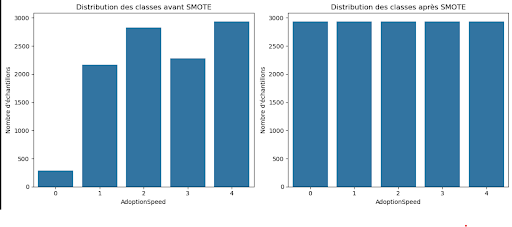
\includegraphics[width=0.8\textwidth]{distribution_smote.png}

    \caption{Distribution des classes avant (gauche) et après (droite) SMOTE}

    \label{fig:smote_distribution}

\end{figure}
 
\vspace{0.5em}

\noindent\textbf{Comparaison des performances avant et après SMOTE}
 
Les deux matrices de confusion ci-dessous comparent les performances du modèle avant et après l’équilibrage des classes. Sur le jeu de test original (non équilibré), le modèle montre un fort biais vers les classes fréquentes, comme 2 et 4. Après application de SMOTE, la répartition des prédictions devient plus homogène, traduisant une amélioration sur les classes minoritaires.
 
\begin{figure}[H]

    \centering

    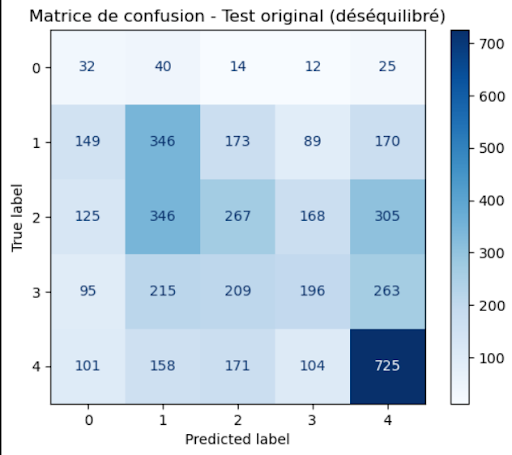
\includegraphics[width=0.45\textwidth]{matrice_confusion_avant_smote.png}

    \hfill

    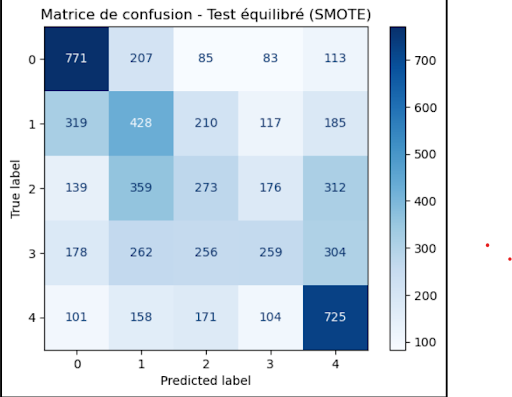
\includegraphics[width=0.45\textwidth]{matrice_confusion_apres_smote.png}

    \caption{Matrice de confusion avant (gauche) et après (droite) SMOTE}

    \label{fig:smote_matrices}

\end{figure}
 
 
\begin{table}[H]

\centering
 
\begin{tabular}{|l|c|c|}

\hline

\textbf{Métrique} & \textbf{Avant SMOTE} & \textbf{Après SMOTE} \\

\hline

Précision (Precision) & 0.3679 & 0.3847 \\

Rappel (Recall)       & 0.3505 & 0.3969 \\

F1-score              & 0.3487 & 0.3835 \\

\hline

\end{tabular}

\caption{Comparaison des performances avant et après application de SMOTE}

\end{table}
 
 
Malgré une légère amélioration des performances suite à l'application de la technique de suréchantillonnage SMOTE, les résultats globaux restent faibles, ce qui indique que le modèle est encore en situation de sous-apprentissage (underfitting). Avant l’utilisation de SMOTE, les métriques de performance sur l’ensemble de test étaient les suivantes : précision de 0.3679, rappel de 0.3505, et F1-score de 0.3487. Après SMOTE, ces valeurs ont légèrement progressé pour atteindre respectivement 0.3847, 0.3969 et 0.3835. Cette amélioration reste toutefois modeste et montre que, bien que le modèle prenne un peu mieux en compte les classes minoritaires, il ne parvient toujours pas à bien apprendre les relations complexes présentes dans les données.
 
Ce constat est appuyé par l’analyse biais-variance, effectuée: le biais observé est élevé (1.9731), tandis que la variance reste relativement faible (0.4588), pour une erreur quadratique moyenne (MSE) totale de 2.4320. Cela confirme que le modèle est trop simple pour la tâche, ce qui se traduit par des prédictions approximatives.
 
Ce comportement illustre parfaitement le compromis biais-variance, un principe fondamental en Machine Learning. Ce compromis vise à équilibrer la complexité du modèle et la qualité des prédictions. Un modèle avec un biais élevé, comme c’est le cas ici, est trop simpliste et ne parvient pas à capturer les structures sous-jacentes dans les données. À l’inverse, un modèle avec une variance trop élevée serait trop sensible aux fluctuations de l’échantillon d’apprentissage, ce qui mène à du sur-apprentissage. L’objectif est donc de trouver un modèle capable d’ajuster sa complexité pour obtenir un bon compromis entre biais et variance, permettant ainsi des prédictions fiables et généralisables. Dans notre cas, les résultats indiquent clairement qu’il faut envisager des modèles plus complexes ou enrichir les données d’entrée (feature engineering) pour sortir de cet état de sous-apprentissage.
 

\subsection{Analyse des tendances globales des variables catégorielles}

Les histogrammes ci-dessous présentent la distribution des variables catégoriques \texttt{Type}, \texttt{Gender}, \texttt{MaturitySize}, \texttt{FurLength}, \texttt{Vaccinated}, \texttt{Dewormed} et \texttt{Sterilized} selon les différentes classes de la variable \texttt{AdoptionSpeed}.
 
De manière générale, on remarque une \textbf{homogénéité marquée} des tendances pour la plupart des variables : les répartitions sont très proches d’une classe à l’autre. Par exemple, pour la variable \texttt{Gender}, les catégories \textit{Male} et \textit{Female} dominent, tandis que \textit{Not Specified} reste marginale. Pour \texttt{MaturitySize}, la catégorie \textit{Medium} est largement majoritaire, suivie de \textit{Small}, alors que \textit{Large} et \textit{Extra Large} sont très peu représentées. La variable \texttt{FurLength} suit une tendance similaire, avec une prédominance des longueurs \textit{Short} et \textit{Medium}, et très peu d’animaux à \textit{Long} pelage.
 
Quant aux variables \texttt{Vaccinated}, \texttt{Dewormed} et \texttt{Sterilized}, les réponses \textit{Yes} et \textit{No} représentent l'essentiel des cas, la modalité \textit{Not Sure} étant beaucoup plus rare.
 
Cependant, on note une \textbf{différence légèrement plus marquée} pour deux variables en particulier : \texttt{Type} et \texttt{Vaccinated}. Pour la variable \texttt{Type}, on observe une proportion légèrement plus élevée de chats (\texttt{Type = 2}) dans les classes d’adoption rapide (classes 0, 1, 2), tandis que les chiens (\texttt{Type = 1}) semblent plus représentés dans les classes d’adoption plus lente (classes 3 et 4). En ce qui concerne la variable \texttt{Vaccinated}, les animaux \textbf{non vaccinés sont majoritaires dans les classes 0, 1 et 2}, tandis que les \textbf{animaux vaccinés sont plus nombreux dans les classes 3 et 4}.
 
Ces observations suggèrent que \textbf{les variables \texttt{Type} et \texttt{Vaccinated} pourraient avoir un potentiel discriminant intéressant}, contrairement aux autres variables catégoriques qui montrent une distribution similaire quel que soit le niveau de \texttt{AdoptionSpeed}. Cela pourrait en faire des \textbf{leviers importants dans la modélisation prédictive}, en aidant à mieux séparer les différentes classes d’adoption dans les futures approches de classification.
\begin{figure}[H]
    \centering
    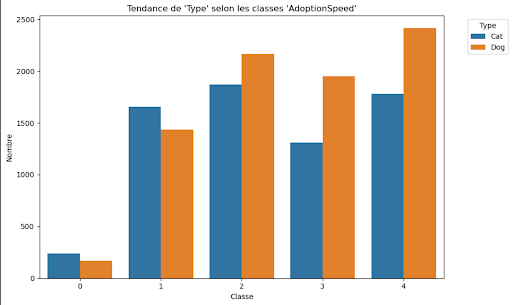
\includegraphics[width=0.75\textwidth]{type_adoption_trend.png}
    \caption{Tendance de la variable \texttt{Type} selon les classes d'\texttt{AdoptionSpeed}}
    \label{fig:type_trend}
\end{figure}

\begin{figure}[H]
    \centering
    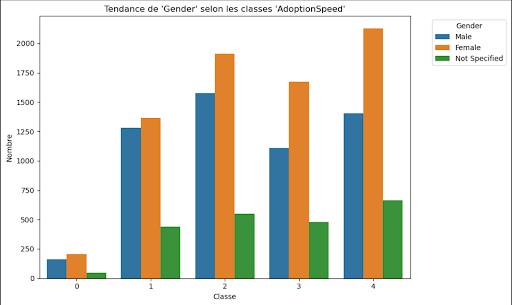
\includegraphics[width=0.75\textwidth]{gender_adoption_trend.png}
    \caption{Tendance de la variable \texttt{Gender} selon les classes d'\texttt{AdoptionSpeed}}
    \label{fig:gender_trend}
\end{figure}

\begin{figure}[H]
    \centering
    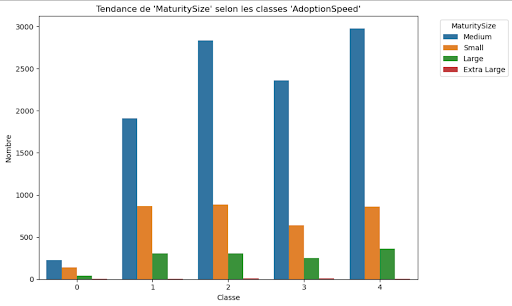
\includegraphics[width=0.75\textwidth]{maturitysize_adoption_trend.png}
    \caption{Tendance de la variable \texttt{MaturitySize} selon les classes d'\texttt{AdoptionSpeed}}
    \label{fig:maturitysize_trend}
\end{figure}

\begin{figure}[H]
    \centering
    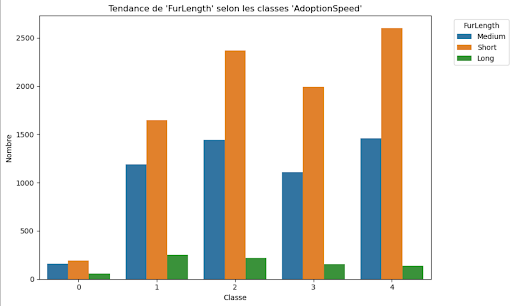
\includegraphics[width=0.75\textwidth]{furlength_adoption_trend.png}
    \caption{Tendance de la variable \texttt{FurLength} selon les classes d'\texttt{AdoptionSpeed}}
    \label{fig:furlength_trend}
\end{figure}

\begin{figure}[H]
    \centering
    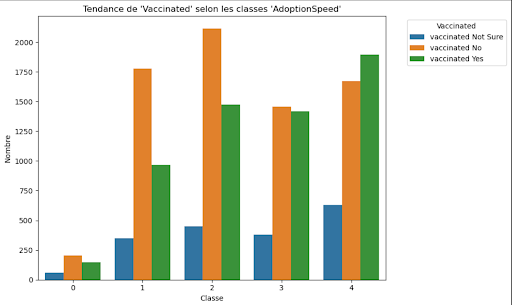
\includegraphics[width=0.75\textwidth]{vaccinated_adoption_trend.png}
    \caption{Tendance de la variable \texttt{Vaccinated} selon les classes d'\texttt{AdoptionSpeed}}
    \label{fig:vaccinated_trend}
\end{figure}

\begin{figure}[H]
    \centering
    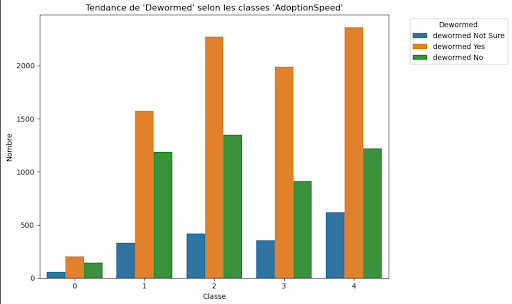
\includegraphics[width=0.75\textwidth]{dewormed_adoption_trend.png}
    \caption{Tendance de la variable \texttt{Dewormed} selon les classes d'\texttt{AdoptionSpeed}}
    \label{fig:dewormed_trend}
\end{figure}

\begin{figure}[H]
    \centering
    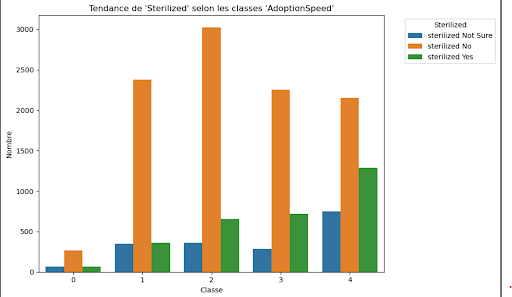
\includegraphics[width=0.75\textwidth]{sterilized_adoption_trend.png}
    \caption{Tendance de la variable \texttt{Sterilized} selon les classes d'\texttt{AdoptionSpeed}}
    \label{fig:sterilized_trend_1}
\end{figure}

\begin{figure}[H]
    \centering
    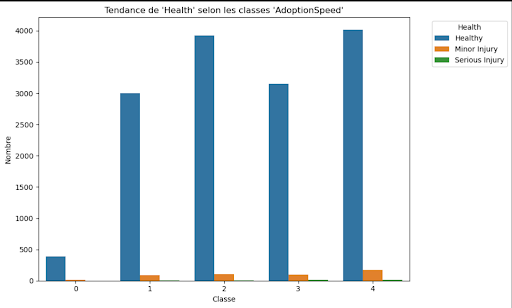
\includegraphics[width=0.75\textwidth]{health_adoption_trend.png}
    \caption{Tendance de la variable \texttt{Health} selon les classes d'\texttt{AdoptionSpeed}}
    \label{fig:health_trend}
\end{figure}

\subsection{Analyse en Composantes Multiples (ACM)}

\subsubsection{Qu’est-ce que l’Analyse des Correspondances Multiples ?}
 
L’\textbf{Analyse des Correspondances Multiples (ACM)} est une méthode d’analyse statistique exploratoire particulièrement adaptée à l’étude de variables qualitatives. Comparable à l’Analyse en Composantes Principales (ACP) qui s’applique aux variables quantitatives, l’ACM permet de représenter visuellement les relations entre les modalités de plusieurs variables catégorielles. Elle projette les données sur un espace à faible dimension — généralement deux ou trois axes — afin de mettre en évidence des proximités, oppositions ou regroupements entre modalités. Cette représentation graphique facilite l’identification de structures sous-jacentes dans les données, telles que des associations typiques entre certaines modalités ou la présence de profils d’observations similaires. L’ACM est ainsi un outil précieux pour simplifier et interpréter des jeux de données complexes, tout en servant souvent de prélude à des analyses plus avancées comme la classification ou la modélisation.
 
Afin de mieux comprendre les relations entre les variables qualitatives du jeu de données, une Analyse en Composantes Multiples (ACM) a été réalisée. Cette méthode permet de visualiser la structure des données catégorielles et d’identifier d’éventuelles associations entre les modalités des différentes variables.
\begin{figure}[H]

    \centering

    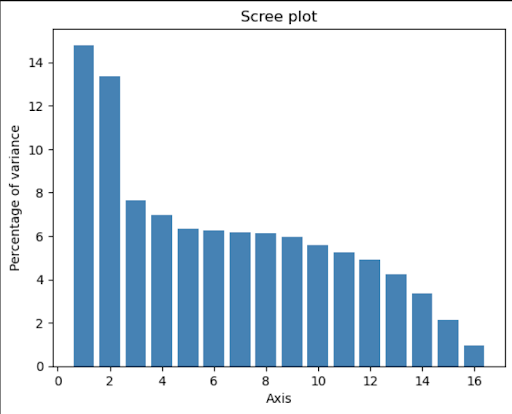
\includegraphics[width=0.7\textwidth]{acm_variance.png}

    \caption{Répartition de la variance expliquée par chaque axe de l'ACM (Scree plot)}

    \label{fig:acm_scree}

\end{figure}
 
Le  graphe \ref{fig:acm_scree} montre la répartition de la variance expliquée par chaque axe. On observe que la première dimension (Dim 1) explique 14,8\% de la variance totale, et la deuxième (Dim 2) 13,35\%. Ensemble, ces deux axes capturent environ 28\% de l'information globale, ce qui est suffisant pour une visualisation initiale. La décroissance progressive de la variance suggère que les premières dimensions concentrent l’essentiel des variations dans les données.
 
\begin{figure}[H]

    \centering

    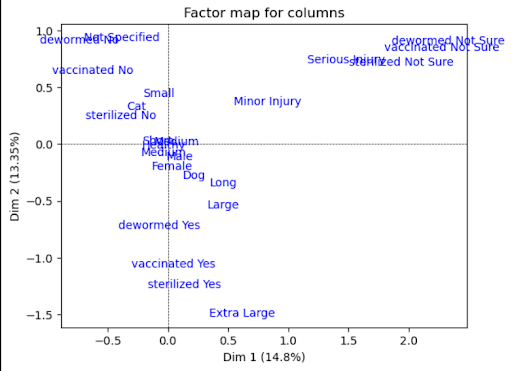
\includegraphics[width=0.8\textwidth]{acm_factor_map.png}

    \caption{Carte factorielle des modalités (ACM)}

    \label{fig:acm_modalites}

\end{figure}
 
La carte factorielle des modalités (Figure~\ref{fig:acm_modalites}) illustre les liens entre les modalités des variables catégorielles. Certaines associations apparaissent clairement :
 
\begin{itemize}

    \item Les modalités \textit{vaccinated YES}, \textit{dewormed YES}, et \textit{sterilized YES} sont regroupées dans le quadrant inférieur gauche, montrant une forte corrélation entre ces traitements sanitaires.

    \item Les modalités opposées \textit{vaccinated NO}, \textit{dewormed NO}, et \textit{sterilized NO} apparaissent ensemble dans le quadrant supérieur gauche.

    \item Un groupe particulier est formé par les modalités \textit{vaccinated NOT SURE}, \textit{dewormed NOT SURE}, et \textit{sterilized NOT SURE}, dans le quadrant supérieur droit.

    \item Les modalités liées au genre (\textit{Male} et \textit{Female}) et à la taille (\textit{Medium}, \textit{Small}, \textit{Large}, \textit{Extra Large}) sont proches de l’origine. Cela indique une faible contribution discriminante sur les deux premiers axes.

\end{itemize}
 
Ces observations confirment les résultats des histogrammes présentés précédemment : les tendances sont globalement homogènes entre les classes d’\textit{AdoptionSpeed}, et aucune variable catégorielle n’émerge clairement comme discriminante. Cela illustre la complexité du problème de classification et justifie le recours à des regroupements de classes pour faciliter l’apprentissage.
 
 
\subsection{selection des variables :}
 
Dans le cadre de notre étude, l'\textbf{Analyse des Correspondances Multiples (ACM)} a permis d’identifier plusieurs variables présentant une dispersion notable sur le plan factoriel. Cela indique qu’elles contribuent significativement à la structuration des individus et pourraient jouer un rôle central dans un futur modèle prédictif. Parmi les variables les plus influentes figurent le \texttt{Type} d’animal, qui distingue entre chiens et chats et peut impacter les comportements d’adoption, ainsi que le statut \texttt{Vaccinated} et \texttt{Dewormed}, qui sont des indicateurs de santé susceptibles d’influencer la perception des adoptants. De même, la variable \texttt{Sterilized} --- critère souvent pris en compte lors d’une adoption --- ressort comme déterminante, tout comme la \texttt{MaturitySize} (taille à maturité) et le niveau de \texttt{Health} (santé), deux éléments particulièrement importants pour les futurs propriétaires.
 
La disposition de ces variables dans le graphe factoriel de l’ACM souligne leur contribution à la variabilité observée entre individus, justifiant leur intégration dans les étapes ultérieures de modélisation. Afin d’enrichir davantage notre approche, nous avons également introduit des variables dérivées comme \texttt{PureBreed}, une variable binaire indiquant si l’animal est de race pure (valeur 1) ou non. Cette distinction peut être déterminante dans la décision d’adoption, certaines races étant perçues comme plus attrayantes ou prestigieuses. Ces ajouts visent à affiner la compréhension des préférences des adoptants tout en améliorant la performance des modèles prédictifs.

 

\subsection{Analyse des clusters : vers une réduction du nombre de classes}

Dans le cadre de notre étude, une analyse de clustering non supervisé a été réalisée afin d’évaluer la cohérence des classes d’adoption existantes dans les données. Pour cela, nous avons utilisé l’algorithme \textit{K-Means}, appliqué aux données préalablement standardisées. Une réduction de dimension par \textbf{ACM}  a été effectuée pour projeter les observations sur deux axes principaux, notés \textit{Composante principale 1} et \textit{Composante principale 2}. Ces deux axes représentent les directions dans lesquelles les données varient le plus, ce qui permet de mieux visualiser la structure des groupes.

Deux configurations ont été testées : un clustering en \textbf{5 groupes} et un clustering en \textbf{2 groupes}.

\begin{figure}[H]
    \centering
    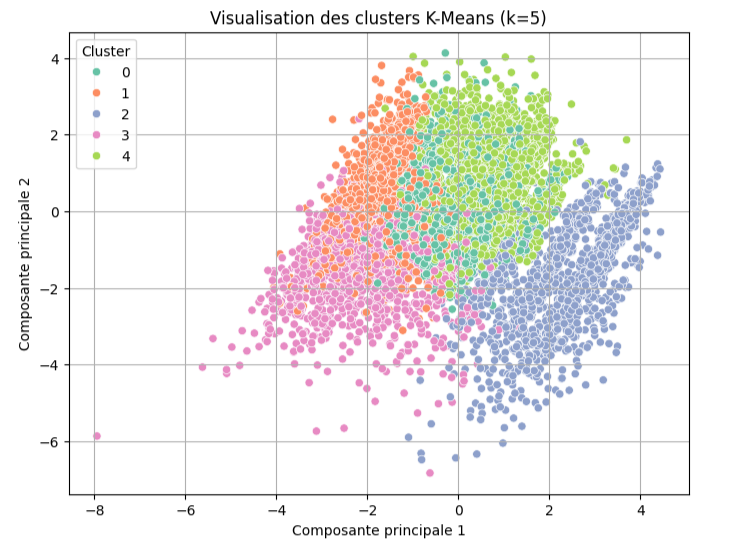
\includegraphics[width=0.7\textwidth]{graph_kmeans_5.png}
    \caption{Clustering KMeans avec $k=5$}
    \label{fig:kmeans_5}
\end{figure}

\begin{figure}[H]
    \centering
    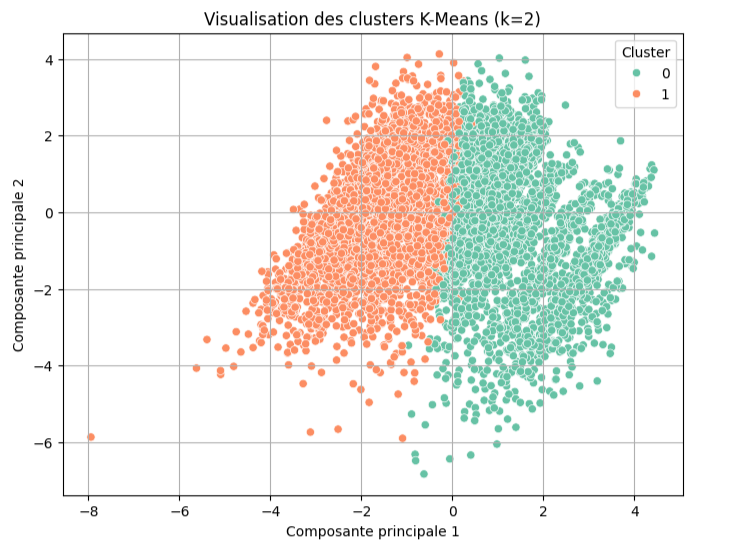
\includegraphics[width=0.7\textwidth]{graph_kmeans_2.png}
    \caption{Clustering KMeans avec $k=2$}
    \label{fig:kmeans_2}
\end{figure}

Le graphe avec $k=5$ montre un chevauchement important entre les groupes, ce qui suggère que la distinction entre les 5 catégories d’adoption n’est pas clairement définie dans l’espace des données. À l’inverse, la représentation avec $k=2$ montre des groupes bien séparés, suggérant qu’un découpage en \textbf{deux catégories globales} serait plus pertinent. Cela renforce l’idée que le problème de prédiction est sans doute mal posé avec 5 classes trop proches ou arbitraires, et qu’un regroupement permettrait une classification plus robuste.

\subsubsection{Analyse des clusters : Répartition de la variable \textit{AdoptionSpeed}}

Afin d’évaluer si les clusters formés par l’algorithme de K-Means correspondent à des profils comportementaux différents vis-à-vis de la vitesse d’adoption, nous avons visualisé la répartition de la variable \textit{AdoptionSpeed} dans chacun des cinq clusters obtenus. Le graphique ci-dessous montre la proportion de chaque classe (0 à 4) au sein de chaque groupe.

\begin{figure}[H]
    \centering
    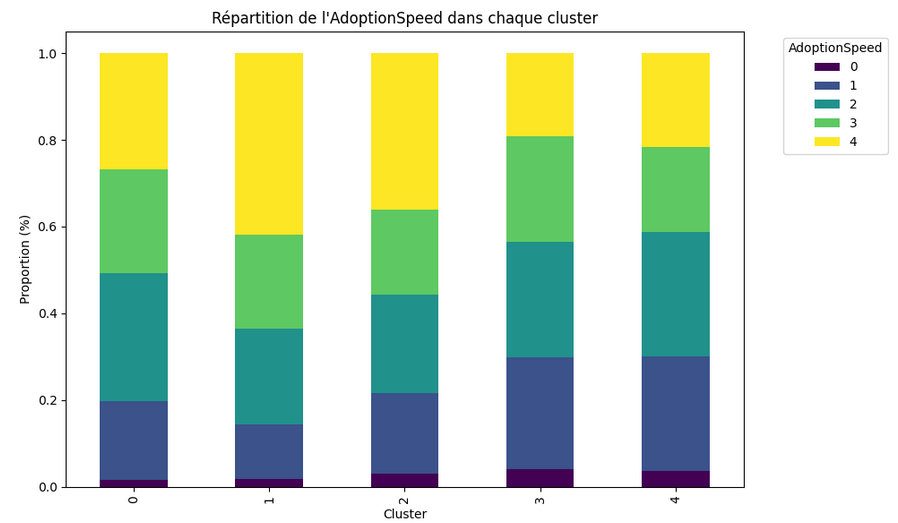
\includegraphics[width=0.75\textwidth]{repartition_de_adoptionspeed.png}
    \caption{Répartition de la variable \textit{AdoptionSpeed} dans chacun des 5 clusters (k=5)}
    \label{fig:cluster_adoption_split}
\end{figure}

On constate que toutes les classes d’\textit{AdoptionSpeed} sont représentées dans chaque cluster, avec des proportions relativement similaires d’un cluster à l’autre. Par exemple, la classe 4 (correspondant à une adoption lente) est présente dans chacun des groupes, parfois légèrement dominante comme dans le cluster 1. Les classes 2 et 3 sont également bien réparties, tandis que la classe 0 reste très minoritaire dans tous les cas.

Cette homogénéité suggère que les variables utilisées pour le clustering (âge, race, couleur, stérilisation, etc.) ne suffisent pas à segmenter efficacement les animaux selon leur rapidité d’adoption. Autrement dit, les regroupements trouvés par K-Means ne révèlent pas de profils très distincts en termes de vitesse d’adoption. Cela renforce la pertinence d’une transformation binaire du problème de classification (par exemple en regroupant certaines classes), comme exploré dans les étapes suivantes de notre analyse.

Afin d'explorer davantage la structure des données, une classification non supervisée en deux clusters a été réalisée.

\begin{figure}[H]
    \centering
    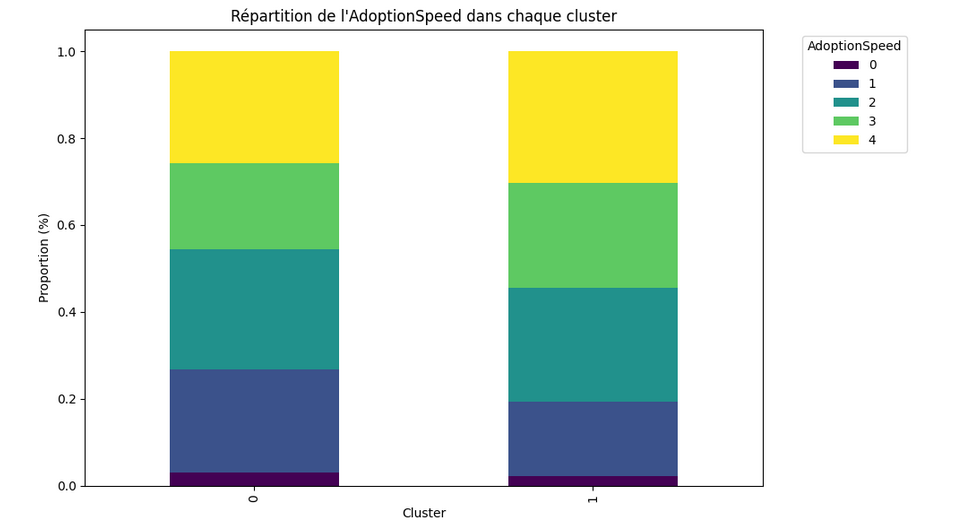
\includegraphics[width=0.7\textwidth]{repartition_adoptionspeed_2clusters.png}
    \caption{Répartition de l'AdoptionSpeed dans les deux clusters}
    \label{fig:repartition_adoptionspeed_2clusters}
\end{figure}

Cependant, l'analyse de la répartition d'\textit{AdoptionSpeed} au sein de ces deux clusters montre que les proportions des différentes classes restent relativement proches d'un cluster à l'autre.

En effet :
\begin{itemize}
    \item Les classes 1, 2, 3 et 4 sont présentes de manière assez homogène dans les deux groupes.
    \item Le cluster 1 présente une légère surreprésentation des animaux non adoptés (classe 4), mais la différence est faible.
\end{itemize}

\textbf{Conclusion :} Ce regroupement en deux clusters n'apporte pas une séparation marquée entre les profils d'animaux rapidement adoptés et ceux non adoptés. Il ne permet donc pas d'améliorer significativement la compréhension ou la prédiction du comportement d'adoption dans ce cas.



\subsection{Traitement des variables \textit{Breed1} et \textit{Type}}
 
Dans notre analyse, nous avons d'abord utilisé un \textbf{arbre de décision simple} pour \textbf{visualiser les décisions prises par le modèle} avant d'envisager des modèles plus avancés tels que le \textbf{Gradient Boosting} ou \textbf{CatBoost}, qui s'appuient également sur des arbres.
 
L'arbre a montré que les \textbf{premiers nœuds} reposaient principalement sur la variable \textit{Breed1} (race de l'animal), avec par exemple des conditions du type \textit{Breed1} $\leq$ 306.5, tandis que la variable \textit{Type} (1 = chien, 2 = chat) n'apparaissait qu'à des niveaux inférieurs de l'arbre.
 
\begin{figure}[H]

    \centering

    \includegraphics[width=0.65\textwidth]{3_premier_noeud_adéciciosn.png}

    \caption{Visualisation des trois premiers nœuds de l'arbre de décision}

    \label{fig:catboost12_conf}

\end{figure}
 
\begin{figure}[H]

    \centering

    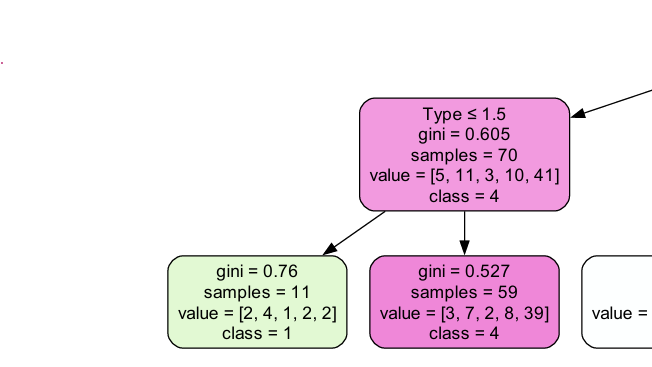
\includegraphics[width=0.65\textwidth]{plus bas dans arbre de decision.png}

    \caption{Structure détaillée des niveaux inférieurs de l'arbre de décision}

    \label{fig:catboost12_conf}

\end{figure}
 
 
Cela soulève plusieurs problèmes :
 
\begin{itemize}

    \item \textbf{Corrélation entre \textit{Breed1} et \textit{Type}} : certaines races sont spécifiques aux chiens, d'autres aux chats. Le modèle peut donc déduire le type d'animal uniquement à partir de la race, sans utiliser explicitement la variable \textit{Type}.

    \item \textbf{\textit{Breed1} est un identifiant arbitraire} : les valeurs numériques associées aux races n'ont pas de signification ordinale. Utiliser cet identifiant brut introduit donc un biais artificiel dans l'apprentissage du modèle.

    \item \textbf{Mauvaise hiérarchisation des décisions} : la variable \textit{Type}, qui est une information binaire essentielle, aurait dû être utilisée dès les premiers niveaux de l'arbre pour séparer clairement les chiens et les chats, facilitant ainsi l'apprentissage de règles plus pertinentes par la suite.

\end{itemize}
 
\bigskip
 
\textbf{Solution proposée :} Pour corriger ce problème, nous avons :
 
\begin{itemize}

    \item Créé des colonnes spécifiques selon le type d'animal : \textit{breed1\_chien}, \textit{breed1\_chat}, \textit{breed2\_chien}, \textit{breed2\_chat}. 

    \item Lorsqu'une colonne ne correspond pas au type de l'animal (par exemple, \textit{breed1\_chat} pour un chien), nous attribuons une valeur fortement pénalisante (par exemple, $-1000$) pour éviter toute confusion lors de l'apprentissage.

    \item Supprimé les variables originales \textit{Breed1} et \textit{Breed2} afin d'éviter que le modèle n'apprenne à partir d'un encodage arbitraire.

\end{itemize}
 
\bigskip
 
\textbf{Avantages attendus :} Cette transformation explicite oblige le modèle à utiliser d'abord la variable \textit{Type}, rendant les règles d'apprentissage plus logiques et réduisant le biais lié à l'ordre arbitraire des races.
 

\subsection{Comparaison de regroupements de classes avec Random Forest}

Afin de mieux comprendre le comportement du modèle, nous avons appliqué une classification binaire en testant deux stratégies de regroupement des classes de la variable \textit{AdoptionSpeed}.

\subsubsection*{Regroupement 1 : (0, 1, 2) vs (3, 4)}

Dans cette première approche, les classes 0, 1 et 2 ont été fusionnées en une classe unique représentant une adoption rapide, tandis que les classes 3 et 4 ont été regroupées sous la classe représentant une adoption lente ou une non-adoption.

Le modèle Random Forest obtient une \textbf{accuracy de 61.27\%}, une \textbf{précision pondérée de 0.6128}, un \textbf{rappel pondéré de 0.6128}, un \textbf{f1-score pondéré de 0.6127}, un \textbf{MSE de 0.3857}, un \textbf{biais de 0.2829} et une \textbf{variance de 0.1028}. La validation croisée donne une moyenne d’accuracy de \textbf{62.55\%}.

\begin{figure}[H]
    \centering
    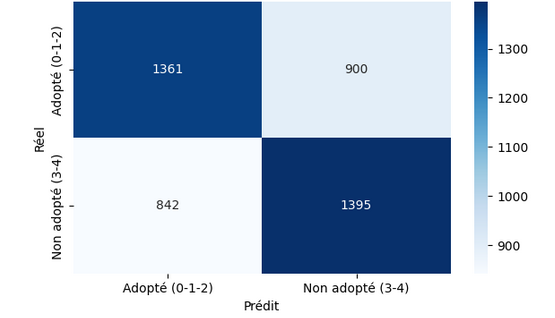
\includegraphics[width=0.7\linewidth]{matrice1.png}
    \caption{Matrice de confusion - Regroupement (0,1,2) vs (3,4)}
    \label{fig:rf_confusion_groupe012}
\end{figure}

\subsubsection*{Regroupement 2 : (1, 2) vs (3, 4)}

Dans une seconde configuration, la classe 0 a été exclue car très peu représentée. Les classes 1 et 2 (adoption modérée à rapide) ont été regroupées, et comparées aux classes 3 et 4 (adoption lente à inexistante).

Avec cette configuration, le modèle obtient une \textbf{accuracy de 60.86\%}, une \textbf{précision pondérée de 0.6085}, un \textbf{rappel pondéré de 0.6086}, un \textbf{f1-score pondéré de 0.6085}, un \textbf{MSE de 0.394}, un \textbf{biais de 0.2912} et une \textbf{variance de 0.1028}. La moyenne en validation croisée est de \textbf{62.57\%}, très proche de la première configuration.

\begin{figure}[H]
    \centering
    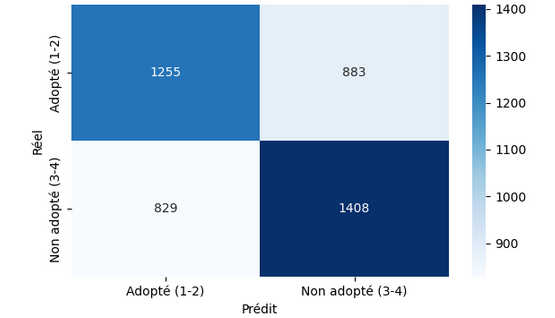
\includegraphics[width=0.7\linewidth]{matrice2.png}
    \caption{Matrice de confusion - Regroupement (1,2) vs (3,4)}
    \label{fig:rf_confusion_groupe12}
\end{figure}

\subsubsection*{Comparaison des deux regroupements}

\begin{table}[H]
    \centering
    \begin{tabular}{|l|c|c|}
        \hline
        \textbf{Critères}    & \textbf{(0,1,2) vs (3,4)} & \textbf{(1,2) vs (3,4)} \\
        \hline
        Accuracy             & 61.27\%                   & 60.86\%                 \\
        Précision (pondérée) & 0.6128                    & 0.6085                  \\
        Rappel (pondéré)     & 0.6128                    & 0.6086                  \\
        F1-score (pondéré)   & 0.6127                    & 0.6085                  \\
        MSE                  & 0.3857                    & 0.394                   \\
        Biais                & 0.2829                    & 0.2912                  \\
        Variance             & 0.1028                    & 0.1028                  \\
        Moyenne CV           & 0.6255                    & 0.6257                  \\
        \hline
    \end{tabular}
    \caption{Comparaison des performances selon deux regroupements de classes}
    \label{tab:rf_comparaison_regroupements}
\end{table}

Les deux stratégies donnent des résultats très similaires. Le regroupement (0,1,2) vs (3,4) obtient des métriques légèrement supérieures, mais le choix entre les deux peut dépendre de la distribution future des données ou des objectifs métier (ex. : minimiser les faux positifs pour les animaux à risque de non adoption).



\subsection{Comparaison des résultats avec XGBoost sur différents regroupements de classes}
 
Le modèle \textbf{XGBoost}, optimisé pour prédire la vitesse d'adoption des animaux en deux classes (adoption lente et rapide), a été entraîné avec les hyperparamètres optimaux suivants : \texttt{\{colsample\_bytree: 0.7, learning\_rate: 0.005, max\_depth: 8, n\_estimators: 100, reg\_lambda: 3, subsample: 0.8\}}. Il a atteint un \textbf{accuracy moyen de 0.6411} en validation croisée (5-fold) et des performances robustes sur le jeu de test, avec une \textbf{précision de 0.6583}, un \textbf{rappel de 0.6569}, un \textbf{F1-score de 0.6559}, et une \textbf{accuracy d’environ 65.8\,\%}, indiquant une capacité équilibrée à identifier correctement les deux classes tout en limitant les erreurs.
 
L'analyse biais-variance révèle une \textbf{erreur quadratique moyenne (MSE)} de \textbf{0.3541}, avec un \textbf{biais au carré} de \textbf{0.2941} et une \textbf{variance} de \textbf{0.0601}. Dans le cadre du compromis biais-variance, le \textbf{biais élevé (0.2941)} suggère que le modèle, bien qu’efficace, reste \textbf{trop simpliste pour capturer pleinement les relations complexes} des données, ce qui peut expliquer pourquoi l’\textbf{accuracy} et le \textbf{F1-score}, bien qu’améliorés, n’atteignent pas des valeurs plus élevées. La \textbf{faible variance (0.0601)} indique toutefois une excellente stabilité, le modèle généralisant bien sans surapprendre aux données d’entraînement.
 
Pour améliorer l’\textbf{accuracy} et réduire le biais, tout en maintenant l’équité des prédictions afin d’éviter des biais discriminatoires dans l’adoption d’animaux, des stratégies telles que l’ajout de \textbf{caractéristiques pertinentes} ou un \textbf{réglage plus fin de la complexité du modèle} pourraient être envisagées.
 
 
\begin{figure}[H]
    \centering
    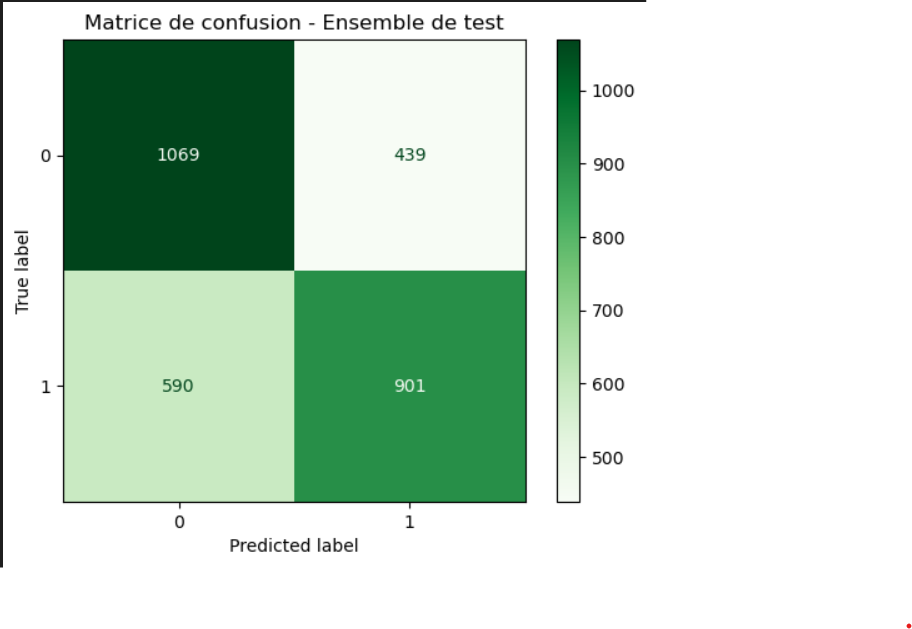
\includegraphics[width=0.8\textwidth]{xgboost0.png}
    \caption{Matrice de confusion - CatBoost (regroupement 0+1+2 vs 3+4)}
    \label{fig:catboost012_conf}
\end{figure}
 
 
 
\begin{table}[h]
\centering
\begin{tabular}{|c|c|c|c|c|c|c|}
\hline
\textbf{validation croisée} & \textbf{Précision} & \textbf{Rappel} & \textbf{F1-score} & \textbf{MSE} & \textbf{Biais} & \textbf{Variance} \\
\hline
0.6411& 0.6582 & 0.6568 & 0.6559 & 0.3541&  0.2941 &  0.0601 \\
\hline
\end{tabular}
\caption{Résultats du modèle XGBoost (regroupement 0+1+2 vs 3+4)}
\end{table}
 
\paragraph{Analyse des performances du modèle XGBoost (Regroupement des classes 1+2 et 3+4)}

Après avoir regroupé les classes 1 et 2 (adoption rapide) ainsi que les classes 3 et 4 (adoption lente), tout en excluant les observations associées à la classe 0, le modèle \textbf{XGBoost} a été optimisé à l’aide des hyperparamètres suivants :
 
\begin{center}

\texttt{\{'colsample\_bytree': 0.7, 'learning\_rate': 0.05, 'max\_depth': 6, 'n\_estimators': 200, 'reg\_lambda': 2, 'subsample': 1.0\}}

\end{center}
 
Ce modèle a atteint une \textbf{précision macro moyenne de 0.6476} lors d'une validation croisée en 5 plis (5-fold), ce qui témoigne d'une performance globale équilibrée.
 
\medskip
 
Sur le jeu de test, les résultats sont les suivants :

\begin{itemize}

    \item \textbf{Précision (precision)} : 0.6425

    \item \textbf{Rappel (recall)} : 0.6407

    \item \textbf{F1-score} : 0.6404

    \item \textbf{Accuracy} : environ 64.2 \%

\end{itemize}
 
Ces performances restent équilibrées, bien qu’un peu inférieures à celles observées dans la configuration précédente (regroupement des classes 0+1+2 et 3+4).
 
\subsection*{Analyse biais-variance}
 
L’analyse biais-variance apporte des informations complémentaires sur le comportement du modèle :
 
\begin{itemize}

    \item \textbf{Erreur quadratique moyenne (MSE)} : 0.3681

    \item \textbf{Biais au carré (Bias$^2$)} : 0.3032

    \item \textbf{Variance} : 0.0649

\end{itemize}
 
Le \textbf{biais élevé} ($0.3032$) indique que le modèle est encore trop simpliste pour représenter correctement les relations complexes présentes dans les données, ce qui freine l'amélioration des performances telles que l’accuracy et le F1-score.
 
En revanche, la \textbf{variance modérée} ($0.0649$), bien que légèrement plus élevée que dans la configuration précédente, reste acceptable. Elle reflète une certaine sensibilité aux fluctuations des données d’apprentissage, mais sans provoquer de surapprentissage manifeste.
 
\subsection*{Conclusion}
 
Ce compromis biais-variance met en évidence une \textbf{stabilité raisonnable} du modèle, mais également une marge d’amélioration possible. Pour mieux capturer la complexité du phénomène d’adoption.
 
 
\begin{figure}[H]

    \centering

    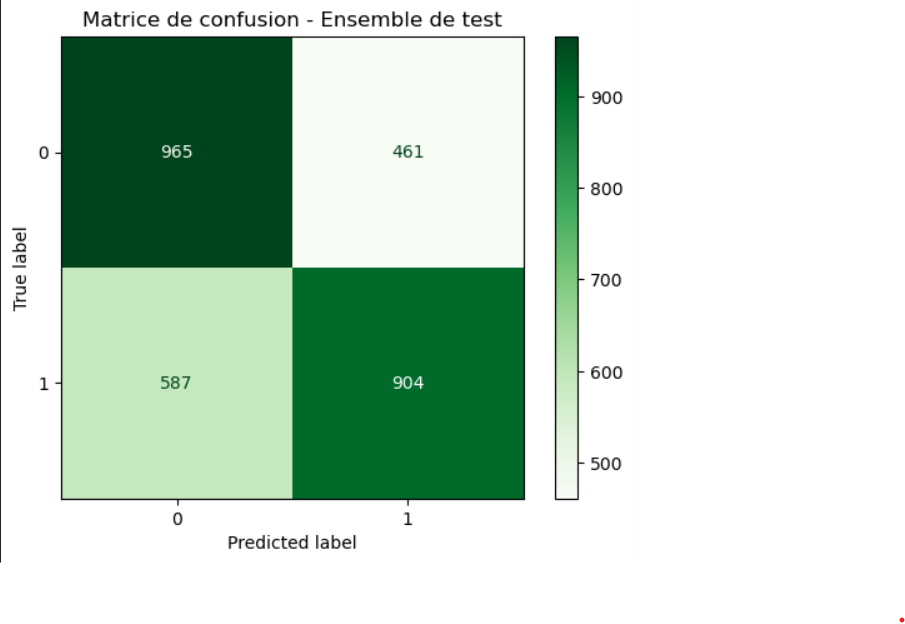
\includegraphics[width=0.8\textwidth]{xgboost1.png}

    \caption{Matrice de confusion - CatBoost (regroupement 1+2 vs 3+4)}

    \label{fig:catboost012_conf}

\end{figure}
 
 
\begin{table}[h]

\centering

\begin{tabular}{|c|c|c|c|c|c|c|}

\hline

\textbf{Validation croisée} & \textbf{Précision} & \textbf{Rappel} & \textbf{F1-score} & \textbf{MSE} & \textbf{Biais} & \textbf{Variance} \\

\hline

0.6476 & 0.6425 & 0.6407 & 0.6404 & 0.3681 & 0.3032 & 0.0649 \\

\hline

\end{tabular}

\caption{Résultats du modèle XGBoost (regroupement 1+2 vs 3+4, classe 0 exclue)}

\end{table}

 

\subsection{Comparaison des combinaisons avec Gradient Boosting}
 
Nous avons testé plusieurs regroupements des classes afin d'évaluer leur impact sur les performances du modèle Gradient Boosting. Deux regroupements ont été analysés :
 
\begin{itemize}

    \item \textbf{Regroupement 1} : (0,1,2) vs (3,4)

    \item \textbf{Regroupement 2} : (1,2) vs (3,4)

\end{itemize}
 
\bigskip
 
Les performances obtenues pour chaque combinaison sont présentées dans le tableau suivant :
 
\begin{table}[H]

\centering

\begin{tabular}{|c|c|c|}

\hline

\textbf{Métrique} & \textbf{(0,1,2) vs (3,4)} & \textbf{(1,2) vs (3,4)} \\ \hline

Précision globale & 0.6636 & 0.6637 \\ \hline

F1-score (Classe 0) & 0.67 & 0.65 \\ \hline

F1-score (Classe 1) & 0.62 & 0.63 \\ \hline

Validation croisée & 0.6470 & 0.6452 \\ \hline

\end{tabular}

\caption{Comparaison des performances des regroupements}

\end{table}
 
\bigskip
 
L'analyse des erreurs montre :
 
\begin{table}[H]

\centering

\begin{tabular}{|c|c|c|}

\hline

\textbf{Métrique} & \textbf{(0,1,2) vs (3,4)} & \textbf{(1,2) vs (3,4)} \\ \hline

Biais & 0.2996 & 0.3050 \\ \hline

Variance & 0.0553 & 0.0599 \\ \hline

MSE & 0.3549 & 0.3649 \\ \hline

\end{tabular}

\caption{Analyse du biais, de la variance et de l'erreur}

\end{table}
 
\bigskip
 
Les matrices de confusion permettent de mieux comprendre les erreurs du modèle :
 
\begin{table}[H]

\centering

\begin{tabular}{|c|c|c|}

\hline

\textbf{Vrai/Prédit} & 0 & 1 \\ \hline

\textbf{Réel 0} & 1063 & 445 \\ \hline

\textbf{Réel 1} & 613 & 878 \\ \hline

\end{tabular}

\caption{Matrice de confusion pour le regroupement (0,1,2) vs (3,4)}

\end{table}
 
\bigskip
 
\begin{table}[H]

\centering

\begin{tabular}{|c|c|c|}

\hline

\textbf{Vrai/Prédit} & 0 & 1 \\ \hline

\textbf{Réel 0} & 969 & 457 \\ \hline

\textbf{Réel 1} & 589 & 902 \\ \hline

\end{tabular}

\caption{Matrice de confusion pour le regroupement (1,2) vs (3,4)}

\end{table}
 
\bigskip
 
 
L'analyse comparative met en évidence que \textbf{la combinaison (0,1,2) vs (3,4) est la meilleure}, car :
 
\begin{itemize}

    \item \textbf{Meilleur F1-score pour la classe 0} (0.67 vs 0.65), améliorant la capacité du modèle à identifier correctement les cas négatifs.

    \item \textbf{Précision légèrement plus fiable en validation croisée} (0.6470 vs 0.6452).

    \item \textbf{Biais et variance plus faibles}, assurant une meilleure stabilité du modèle.

    \item \textbf{Moins d'erreurs sur la classe 0}, ce qui améliore la robustesse globale du modèle.

\end{itemize}
 
Ainsi, la combinaison \textbf{(0,1,2) vs (3,4)} est \textbf{recommandée} pour obtenir des performances plus équilibrées et une meilleure stabilité du modèle.
 
 
 
\section{ Les descriptions positives accélèrent-elles l’adoption des animaux ?
 }

Dans le cadre de notre projet, nous avons constaté que la variable "description" dans notre jeu de données pourrait avoir un impact sur nos résultats. Nous avons donc décidé d'analyser cette variable et d'examiner l'impact des sentiments exprimés dans les descriptions des animaux sur leur vitesse d'adoption. Pour ce faire, nous utilisons l'outil VADER, qui permet d'analyser automatiquement les descriptions rédigées par les anciens propriétaires. Cet outil génère plusieurs scores de sentiment : positif, négatif, neutre, ainsi qu'un score global composé. Ces scores sont ensuite enregistrés dans un fichier intitulé "sentiment.csv".

L'objectif de cette expérimentation est d'explorer s'il existe une corrélation entre les émotions véhiculées dans les descriptions textuelles et le temps nécessaire à l'adoption d'un animal. En croisant les scores de sentiment avec les délais d'adoption, nous espérons mieux comprendre l'influence de descriptions plus ou moins positives sur le comportement des adoptants potentiels.


\begin{figure}[H]
    \centering
    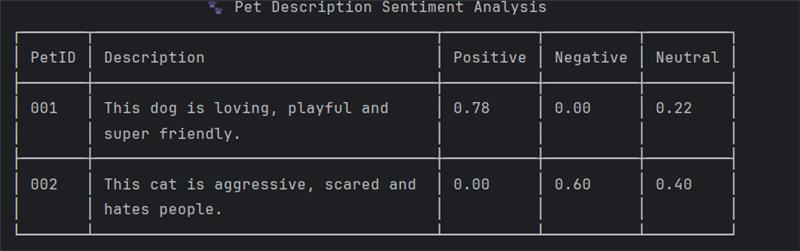
\includegraphics[width=0.8\textwidth]{image.jpg}
    \caption{Exemple d'analyse de sentiment sur des descriptions}
    \label{fig:sentiment}
\end{figure}

 
 
 
 
 
 
\subsection{Ajout des sentiments textuels dans le Gradient Boosting}
 
Après avoir fusionné les classes \textbf{0, 1 et 2} en une classe \textbf{0}, et les classes \textbf{3 et 4} en une classe \textbf{1}, nous avons enrichi notre modèle en y intégrant des variables dérivées de l’analyse textuelle des descriptions des animaux. Ces nouvelles variables correspondent aux scores de sentiment \textit{positif}, \textit{négatif} et \textit{neutre} extraits des textes descriptifs.
 
\bigskip
 
\subsubsection{Performances du Modèle avec Sentiment}
 
\begin{table}[H]

\centering

\begin{tabular}{|c|c|}

\hline

\textbf{Hyperparamètre} & \textbf{Valeur} \\ \hline

Learning Rate & 0.05 \\ \hline

Max Depth & 4 \\ \hline

N Estimators & 200 \\ \hline

\end{tabular}

\caption{Meilleurs hyperparamètres du modèle avec variables de sentiment}

\end{table}
 
\bigskip
 
\textbf{Résultats en validation croisée} :
 
\begin{table}[H]

\centering

\begin{tabular}{|c|c|}

\hline

\textbf{Métrique} & \textbf{Valeur} \\ \hline

Précision moyenne (macro) & 0.6461 \\ \hline

\end{tabular}

\caption{Précision moyenne en validation croisée}

\end{table}
 
\bigskip
 
\textbf{Résultats globaux du modèle (Chiens + Chats)} :
 
\begin{table}[H]

\centering

\begin{tabular}{|c|c|c|c|c|}

\hline

\textbf{Classe} & \textbf{Précision} & \textbf{Rappel} & \textbf{F1-score} & \textbf{Support} \\ \hline

0 & 0.63 & 0.67 & 0.65 & 1426 \\ \hline

1 & 0.66 & 0.62 & 0.64 & 1491 \\ \hline

\end{tabular}

\caption{Performances du modèle avec variables de sentiment}

\end{table}
 
\bigskip
 
\subsubsection{Analyse du biais, de la variance et de l'erreur}
 
\begin{table}[H]

\centering

\begin{tabular}{|c|c|}

\hline

\textbf{Métrique} & \textbf{Valeur} \\ \hline

MSE & 0.3634 \\ \hline

Biais & 0.2975 \\ \hline

Variance & 0.0660 \\ \hline

\end{tabular}

\caption{Analyse du biais et de la variance du modèle avec variables de sentiment}

\end{table}
 
\bigskip
 
\subsubsection{Matrice de confusion}
 
\begin{table}[H]

\centering

\begin{tabular}{|c|c|c|}

\hline

\textbf{Vrai/Prédit} & 0 & 1 \\ \hline

\textbf{Réel 0} & 951 & 475 \\ \hline

\textbf{Réel 1} & 567 & 924 \\ \hline

\end{tabular}

\caption{Matrice de confusion du modèle avec variables de sentiment}

\end{table}
 
\bigskip
 
\subsection{Comparaison entre le modèle avec et sans variables de sentiment}
 
\begin{table}[H]

\centering

\begin{tabular}{|c|c|c|}

\hline

\textbf{Métrique} & \textbf{Sans Sentiment} & \textbf{Avec Sentiment} \\ \hline

Précision globale & 0.6637 & 0.6605 \\ \hline

Précision moyenne (macro) & 0.6452 & 0.6461 \\ \hline

F1-score (Classe 0) & 0.65 & 0.65 \\ \hline

F1-score (Classe 1) & 0.63 & 0.64 \\ \hline

Biais & 0.3050 & 0.2975 \\ \hline

Variance & 0.0599 & 0.0660 \\ \hline

MSE & 0.3649 & 0.3634 \\ \hline

\end{tabular}

\caption{Comparaison des performances du modèle avec et sans variables de sentiment}

\end{table}
 
\bigskip
 
\subsection{Interprétation des résultats}
 
Les résultats montrent que l'ajout des variables de sentiment dans le modèle n'améliore pas significativement les performances :
 
\begin{itemize}

    \item La \textbf{précision globale} diminue légèrement lorsque les variables de sentiment sont ajoutées (0.6605 vs 0.6637).

    \item Le \textbf{F1-score} reste stable, sans amélioration majeure pour les classes 0 et 1.

    \item La \textbf{variance augmente} légèrement (0.0660 vs 0.0599), ce qui indique une instabilité accrue du modèle.

    \item La \textbf{matrice de confusion} montre plus d'erreurs avec le modèle incluant les sentiments, avec une augmentation des faux positifs et faux négatifs.

\end{itemize}
 
\bigskip
 
L'ajout des variables de sentiment textuel ne permet pas d'améliorer les performances du modèle Gradient Boosting. Au contraire, il entraîne une légère dégradation en augmentant la variance et en réduisant la précision.
 
\textbf{Par conséquent, le modèle sera conservé sans les variables de sentiment afin d'assurer une meilleure stabilité et des performances optimales.}

\begin{thebibliography}{9}

    \bibitem{bias_variance_innovatiana}
    Innovatiana, 
    \emph{Bias Estimation in Machine Learning}, 
    [En ligne]. Disponible sur : \url{https://www.innovatiana.com/post/bias-estimation-in-machine-learning#:~:text=Ce%20biais%20survient%20lorsque%20l,pr%C3%A9cises%20pour%20les%20autres%20groupes}. 
    
    \bibitem{xlstat_acm}
    XLSTAT,
    \emph{Analyse des correspondances multiples (ACM ou AFCM)}, 
    [En ligne]. Disponible sur : \url{https://www.xlstat.com/fr/solutions/fonctionnalites/analyse-des-correspondances-multiples-acm-ou-afcm}. 
    
    \bibitem{github_acm}
    Le Coin Stat,
    \emph{100 Jours de Machine Learning - Analyse des correspondances multiples (ACM)}, 
    [GitHub Notebook]. Disponible sur : \url{https://github.com/LeCoinStat/100JoursDeML/blob/main/02_Statistiques_Pour_Le_Machine_Learning/03_ACM/acm.ipynb}. 
    
    \end{thebibliography}
    
    
 
\end{document}
